
% \begin{figure*}[!ht]
%   \centering
%     \includegraphics[width=1.0\linewidth]{Fig/data_statistic.pdf}
%     % \vspace{-1.4em}
%     \caption{ The prompt template used for generating scenario descriptions.
%     }
%     \label{fig:data_statistic}
% \end{figure*}

% \section{Discussion}
% Overall speaking, the extensive experiments reveal that: 

\section{More Details on AgentHallu}
\subsection{Dataset and Code Release}
\label{appendix_data_code_realease}
The dataset and code are distributed under the Creative Commons Attribution-NonCommercial-ShareAlike 4.0 International License (CC BY-NC-SA 4.0). This license permits sharing and adaptation with appropriate attribution for non-commercial use, provided that derivative works are distributed under the same terms.

\subsection{Dataset Statistics}
\label{appendix_data_statis}

\subsubsection{Category Statistics}
AgentHallu includes 693 trajectories across one non-hallucination category and five hallucination categories and fourteen subcategories, with distribution statistics presented in Table~\ref{tab:category_ratio}. As shown in Table~\ref{tab:category_ratio}, the category distribution is intentionally balanced to ensure comprehensive and equitable coverage of diverse hallucination types. 

\begin{table}[h]
    \centering
    \tabcolsep=5pt
    \caption{The statistics of AgentHallu over one non-hallucination category and five hallucination categories and fourteen sub categories.}
    \label{tab:category_ratio}
    \resizebox{\linewidth}{!}{
\begin{tabular}{lrr}
            \toprule
             \textbf{Category}  &\textbf{Samples} & \textbf{Ratio(\%)} \\
             \midrule
             \rowcolor{COLOR_MEAN} 
            \hspace{0.3cm} \textbf{Non-Hallucination} &  \textbf{250} & \textbf{36.1} \\
            \midrule
            \rowcolor{category-S1} 
            \hspace{0.3cm} \textbf{Planning Hallucination} &  \textbf{67} & \textbf{9.7} \\ 
                \hspace{0.6cm} \hspace{0.3cm} $\bullet$ Fact Derive &  37 & 5.3 \\ 
                \hspace{0.6cm} \hspace{0.3cm} $\bullet$ Task Decompose &  30 & 4.3 \\ 
            \rowcolor{category-S2} 
            \hspace{0.3cm} \textbf{Retrieval Hallucination} &  \textbf{82} & \textbf{11.8} \\ 
                \hspace{0.6cm} \hspace{0.3cm} $\bullet$ Query Misalign &  18 & 2.6 \\ 
                \hspace{0.6cm} \hspace{0.3cm} $\bullet$ Context Misalign & 18 & 2.6 \\ 
                \hspace{0.6cm} \hspace{0.3cm} $\bullet$ Summarize Misalign & 46 & 4.6 \\ 
            \rowcolor{category-S3} 
            \hspace{0.3cm} \textbf{Reasoning Hallucination} &  \textbf{118} & \textbf{17.0} \\ 
                \hspace{0.6cm} \hspace{0.3cm} $\bullet$ Factual Reasoning & 18 & 2.6 \\ 
                \hspace{0.6cm} \hspace{0.3cm} $\bullet$ Science Reasoning &  37 & 5.3 \\ 
                \hspace{0.6cm} \hspace{0.3cm} $\bullet$ Math Reasoning &  45 & 6.5 \\ 
                \hspace{0.6cm} \hspace{0.3cm} $\bullet$ General Reasoning &  18 & 2.6 \\ 
             \rowcolor{category-S4} 
            \hspace{0.3cm} \textbf{Human-Interaction Hallucination} &  \textbf{73} & \textbf{10.5} \\ 
            \rowcolor{category-S5} 
            \hspace{0.3cm} \textbf{Tool-Use Hallucination} &  \textbf{103} & \textbf{14.9} \\ 
                \hspace{0.6cm} \hspace{0.3cm} $\bullet$ Missing Required Call & 32 & 4.6 \\ 
                \hspace{0.6cm} \hspace{0.3cm} $\bullet$ Incorrect Tool Arguments &  36 & 5.3 \\
                \hspace{0.6cm} \hspace{0.3cm} $\bullet$ Unnecessary Tool Call &  23 & 3.3 \\ 
                \hspace{0.6cm} \hspace{0.3cm} $\bullet$ Parallel Call Conflict &  12 & 1.6 \\ 
            \bottomrule
        \end{tabular}
    }
\end{table}



















\subsubsection{Word Cloud}
The query distribution in AgentHallu is visualized as a word cloud in Figure~\ref{appendix_word_cloud}. Prevalent high-frequency terms highlight recurring linguistic patterns in agent queries, including tool invocations and information-seeking requests. The breadth of salient keywords indicates substantial topical diversity, suggesting that the benchmark covers a wide range of realistic user intents rather than a narrow set of prompt templates.

\begin{figure}[!t]
  \centering
    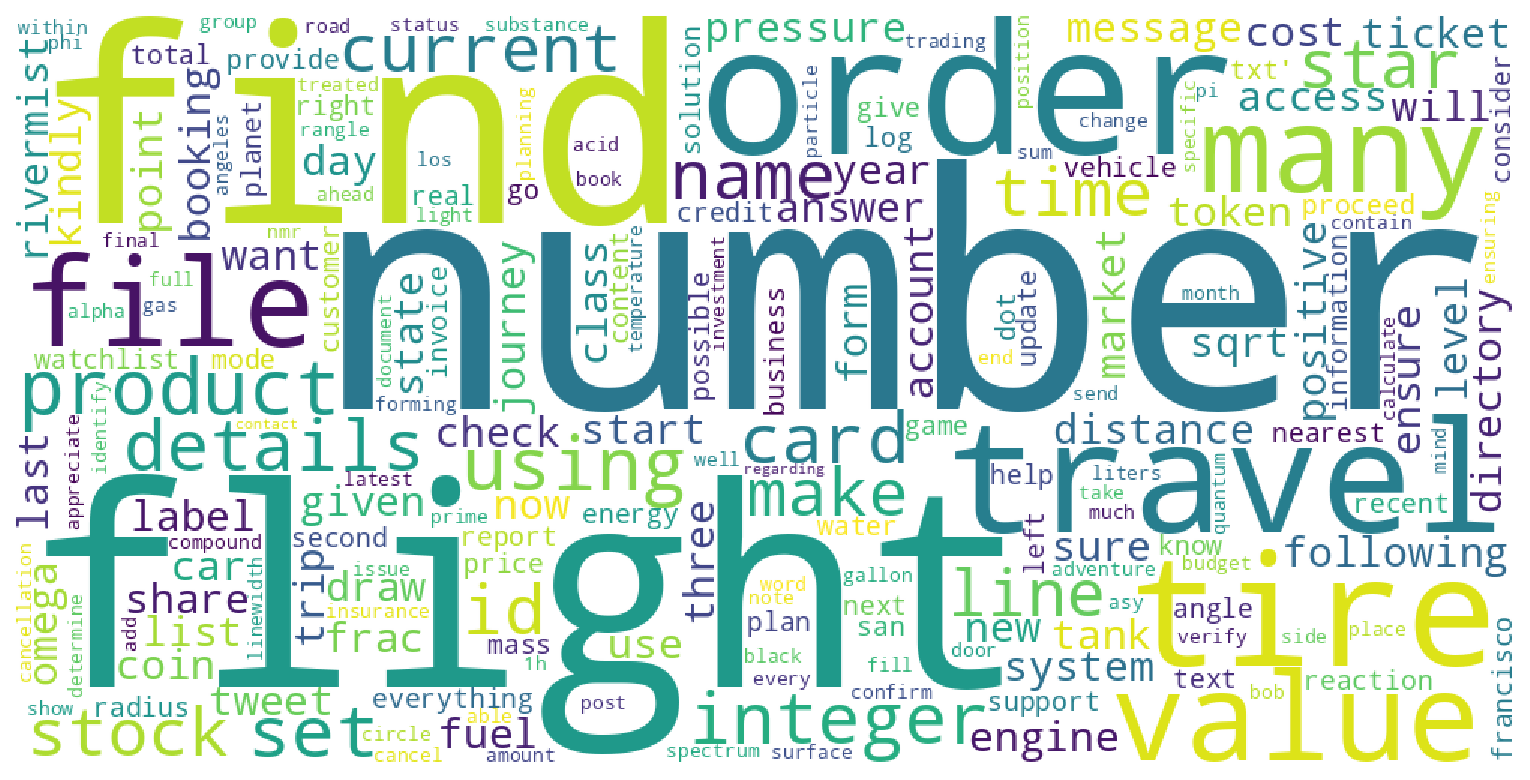
\includegraphics[width=1.0\linewidth]{Fig/word_cloud.pdf}
    % \vspace{-2.0em}
    \caption{ Word cloud of queries in AgentHallu dataset.
    }
    \label{appendix_word_cloud}
\end{figure}

\subsubsection{Trajectory Distribution}
We present the trajectory length distribution of AgentHallu, measured by the number of steps per trajectory in Figure~\ref{appendix_tragectory_step}. As shown in Figure~\ref{appendix_tragectory_step}, AgentHallu excludes overly short trajectories with one or two steps. The longest trajectory contains 43 steps, and lengths are broadly distributed across step counts, indicating substantial diversity in interaction depth and long-horizon reasoning.

\begin{figure}[!ht]
  \centering
    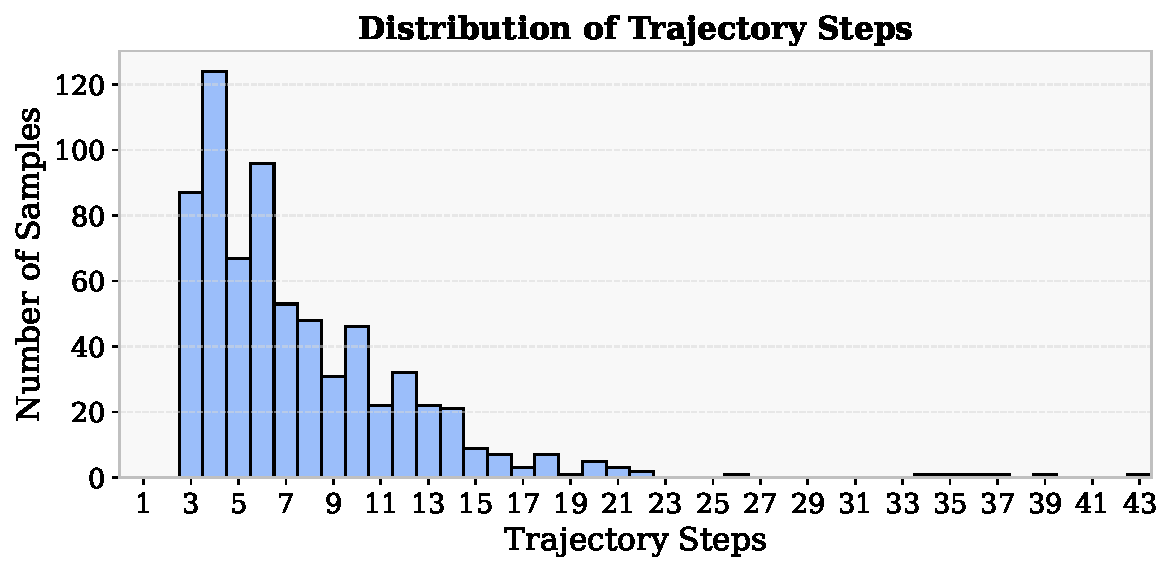
\includegraphics[width=1.0\linewidth]{Fig/history_step_plot.pdf}
    % \vspace{-2.0em}
    \caption{ Distribution of trajectory lengths measured by the number of steps per trajectory.
    }
    \label{appendix_tragectory_step}
\end{figure}

\begin{table*}[t!]
    \centering
    \caption{Distribution of query sources across agent frameworks in AgentHallu.}
        \vspace{-0.5em}
    \label{agent_dataset_distribution}
    \resizebox{\linewidth}{!}{
    \tablestyle{3.0pt}{1.0}
    \begin{tabular}{l||cccccccc|c}
\rowcolor{COLOR_MEAN}
\toprule
\textbf{Agent Framework} & \multicolumn{1}{l}{\textbf{SimpleQA}} & \multicolumn{1}{l}{\textbf{GPQA}} & \multicolumn{1}{l}{\textbf{MATH-500}} & \multicolumn{1}{l}{\textbf{AIME2024}} & \multicolumn{1}{l}{\textbf{AIME2025}} & \multicolumn{1}{l}{\textbf{GAIA}} & \multicolumn{1}{l}{\textbf{HLE}} & \multicolumn{1}{l|}{\textbf{BFCL V3}} & \multicolumn{1}{l}{\textbf{Total}} \\ \midrule \midrule
SmolAgents               & 27                                    & 20                                & 21                                    & 1                                     & 2                                     & 14                                & 6                                & -                                     & 91                                 \\
OpenDeepSearch           & 55                                    & 9                                 & 13                                    & 3                                     & 3                                     & 10                                & 6                                & -                                     & 100                                \\
OpenManus                & 42                                    & 36                                & 8                                     & 7                                     & 7                                     & 4                                 & 0                                & -                                     & 104                                \\
Octotools                & 14                                    & 11                                & 13                                    & 0                                     & 0                                     & 5                                 & 4                                & -                                     & 47                                 \\
Magentic-One             & 28                                    & 25                                & 8                                     & 3                                     & 5                                     & 20                                & 5                                & -                                     & 94                                 \\
OWL                      & 17                                    & 36                                & 13                                    & 2                                     & 7                                     & 15                                & 3                                & -                                     & 93                                 \\ Function-Calling Agent   & -                                     & -                                 & -                                     & -                                     & -                                     & -                                 & -                                & 164                                   & 164                                \\ \midrule \midrule
Total                    & 183                                   & 137                               & 76                                    & 16                                    & 24                                    & 68                                & 25                               & -                                     & 693                                \\ \bottomrule
\end{tabular}
    }
\end{table*}




\subsection{Agent Configuration}

\subsubsection{Agent Description}
\label{appendix_agent_descrip}
We instantiate agent trajectories using seven representative LLM-based agents that span diverse reasoning paradigms and interaction patterns. We briefly summarize each framework below.
\begin{itemize}[noitemsep,left=2pt, itemsep=0pt, topsep=0pt]
    \item \textit{SmolAgents}~\cite{roucher2025smolagents}: SmolAgents is a lightweight agent framework that supports both CodeAct-style~\cite{wang2024executable} and ReAct-style~\cite{yao2022react} agents, and we configure both agent types within our method.
    \item \textit{OpenDeepSearch}~\cite{alzubi2025open}: Built on SmolAgents as the reasoning agent, OpenDeepSearch integrates an advanced search tool that leverages an embedded LLM to refine retrieved context. We also configure both CodeAct-style and ReAct-style agent variants.
    \item \textit{OpenManus}~\cite{openmanus2025}: OpenManus extends the planner–toolcaller architecture by incorporating explicit human-in-the-loop interactions, enabling the agent to solicit user input and integrate feedback during task execution.
    \item \textit{OctoTools}~\cite{lu2025octotools}: OctoTools provides over ten standardized tool cards that encapsulate diverse functionalities, enabling efficient multi-tool workflows for complex computational tasks.
    \item \textit{Magentic-One}~\cite{fourney2024magentic}: Magnetic-One employs a coordinator agent that collaborates with four specialized agents: a WebSurfer agent to browse the web, a FileSurfer agent to handle files, a Coder agent to write code, and a Computer Terminal agent to execute code.
    \item \textit{OWL}~\cite{hu2025owl}: OWL includes a workforce-oriented framework with a Planner for task decomposition, a Coordinator for subtask management, and specialized Workers capable of domain-specific tool invocation.
    \item \textit{Function-calling Agent}~\cite{patilberkeley}: A function-calling agent conditions an LLM on a set of tool or API specifications. The agent then emits a structured function call that selects the appropriate function and fills in its arguments. The tool output is fed back to the agent, enabling multi-turn execution and iterative reasoning.
\end{itemize}

\begin{table}[ht]
    \centering
    \caption{Distribution of LLM backbones across agent frameworks in AgentHallu.}
    \vspace{-0.5em}
    \label{tab:agent_model_distribution}
    \resizebox{\linewidth}{!}{
    \tablestyle{4pt}{1.03}
\begin{tabular}{lrr}
            \toprule
             \textbf{Model Backbone}  &\textbf{Samples} & \textbf{Ratio(\%)} \\
            \midrule
            \rowcolor{COLOR_MEAN} 
            \hspace{0.3cm} \textbf{SmolAgents} &  \textbf{91} & \textbf{13.1} \\ 
                \hspace{0.6cm} \hspace{0.3cm} $\bullet$ GPT-4.1 &  45 & 6.5 \\ 
                \hspace{0.6cm} \hspace{0.3cm} $\bullet$ GPT-4o &  30 & 3.2 \\ 
                \hspace{0.6cm} \hspace{0.3cm} $\bullet$ Claude-3.7-Sonnet &  5 & 0.7 \\
                \hspace{0.6cm} \hspace{0.3cm} $\bullet$ Qwen2.5-Coder-32B &  19 & 2.7 \\
            \rowcolor{COLOR_MEAN} 
            \hspace{0.3cm} \textbf{OpenDeepSearch} &  \textbf{100} & \textbf{14.4} \\ 
                \hspace{0.6cm} \hspace{0.3cm} $\bullet$ GPT-4.1 &  36 & 5.2 \\ 
                \hspace{0.6cm} \hspace{0.3cm} $\bullet$ GPT-4o & 9 & 1.3 \\ 
                \hspace{0.6cm} \hspace{0.3cm} $\bullet$ Claude-3.7-Sonnet & 19 & 2.7 \\
                \hspace{0.6cm} \hspace{0.3cm} $\bullet$ Qwen2.5-Coder-32B &  36 & 5.2 \\
            \rowcolor{COLOR_MEAN} 
            \hspace{0.3cm} \textbf{OpenManus} &  \textbf{104} & \textbf{15.0} \\ 
                \hspace{0.6cm} \hspace{0.3cm} $\bullet$ GPT-4.1 & 40 & 5.8 \\ 
                \hspace{0.6cm} \hspace{0.3cm} $\bullet$ GPT-4o &  40 & 5.8 \\ 
                \hspace{0.6cm} \hspace{0.3cm} $\bullet$ GPT-5 &  17 & 2.5 \\ 
                \hspace{0.6cm} \hspace{0.3cm} $\bullet$ Claude-3.7-Sonnet &  7 & 1.0 \\ 
             \rowcolor{COLOR_MEAN} 
            \hspace{0.3cm} \textbf{Octotools} &  \textbf{47} & \textbf{6.8} \\ 
                \hspace{0.6cm} \hspace{0.3cm} $\bullet$ GPT-4.1 &  13 & 1.9 \\ 
                \hspace{0.6cm} \hspace{0.3cm} $\bullet$ GPT-4o &  34 & 4.9 \\ 
            \rowcolor{COLOR_MEAN} 
            \hspace{0.3cm} \textbf{Magentic-One} &  \textbf{94} & \textbf{13.6} \\ 
                \hspace{0.6cm} \hspace{0.3cm} $\bullet$ GPT-4.1 & 50 & 7.2 \\ 
                \hspace{0.6cm} \hspace{0.3cm} $\bullet$ GPT-4o &  15 & 2.2 \\ 
                \hspace{0.6cm} \hspace{0.3cm} $\bullet$ GPT-5 &  21 & 3.0 \\ 
                \hspace{0.6cm} \hspace{0.3cm} $\bullet$ Claude-3.7-Sonnet &  8 & 1.2 \\ 
            \rowcolor{COLOR_MEAN} 
            \hspace{0.3cm} \textbf{OWL} &  \textbf{93} & \textbf{13.4} \\ 
                \hspace{0.6cm} \hspace{0.3cm} $\bullet$ GPT-4.1 & 72 & 10.4 \\ 
                \hspace{0.6cm} \hspace{0.3cm} $\bullet$ GPT-4o &  4 & 0.6 \\ 
                \hspace{0.6cm} \hspace{0.3cm} $\bullet$ GPT-5 &  17 & 2.5 \\ 
            \rowcolor{COLOR_MEAN} 
            \hspace{0.3cm} \textbf{Function-calling Agent} &  \textbf{164} & \textbf{23.7} \\ 
                \hspace{0.6cm} \hspace{0.3cm} $\bullet$ GPT-4.1 &  60 & 8.7 \\ 
                \hspace{0.6cm} \hspace{0.3cm} $\bullet$ Qwen3-32B &  60 & 8.7 \\ 
                \hspace{0.6cm} \hspace{0.3cm} $\bullet$ Llama3.3-70B &  44 & 6.3 \\
            \bottomrule
        \end{tabular}
    }
\end{table}



















\subsubsection{Agent Distribution across Datasets}
We present the distribution of query dataset sources across agent frameworks in AgentHallu, as shown in Table~\ref{agent_dataset_distribution}. The six general agent frameworks contribute trajectories across all seven knowledge-intensive datasets, yielding broad and relatively balanced coverage. In contrast, the function-calling agent is used exclusively for BFCL V3 queries to assess tool selection and argument filling behavior. Overall, we obtain 693 trajectories spanning heterogeneous agent designs and data sources, suggesting that AgentHallu captures diverse execution patterns and task contexts rather than artifacts of a specific agent implementation.

\begin{table*}[!t]
  \centering
%   \scriptsize
  \caption{Configuration details of LLMs used for trajectory generation and hallucination evaluation in AgentHallu.}
  \label{model_version}
   % \vspace{-1.0em} 
    \resizebox{\linewidth}{!}{
    \tablestyle{5.0pt}{1.1}
   \begin{tabular}{llccc}
\toprule
\textbf{Organization}               & \multicolumn{1}{l}{\textbf{Model}}    & \multicolumn{1}{l}{\textbf{Release}} & \textbf{Version} & \multicolumn{1}{l}{\textbf{Inference Pipeline}} \\ \midrule
\rowcolor{COLOR_MEAN}
\multicolumn{5}{l}{\textit{\textbf{Proprietary LLMs}}}                                    \\ 
\multirow{2}{*}{Google}             & \multicolumn{1}{l}{Gemini 2.5 Pro}  & 2025-6                              & \texttt{gemini-2.5-pro-06-17}                 & API                                             \\
                                    & \multicolumn{1}{l}{Gemini 2.5 Flash}    & 2025-6                                     & \texttt{gemini-2.5-flash-06-17}                   & API                                             \\
\arrayrulecolor{COLOR_MEAN}
\midrule
\arrayrulecolor{black}
\multirow{4}{*}{OpenAI}             & \multicolumn{1}{l}{GPT-5}            & 2025-8                              & \texttt{gpt-5-2025-08-07}                    & API                                             \\
                                    & \multicolumn{1}{l}{GPT-5-mini}       & 2025-8                               & \texttt{gpt-5-mini-2025-08-07}               & API                                             \\
                                    & \multicolumn{1}{l}{GPT-4.1}       & 2025-4                               & \texttt{gpt-4.1-2025-04-14}               & API                                             \\
                                    & \multicolumn{1}{l}{GPT-4o}       & 2024-12                               & \texttt{gpt-4o-2024-11-20}               & API                                             \\
\arrayrulecolor{COLOR_MEAN}
\midrule
\arrayrulecolor{black}
\multirow{2}{*}{Anthropic}          & \multicolumn{1}{l}{Claude-4.5-Sonnet} & 2025-09                              & \texttt{claude-4-5-sonnet-20250929}           & API                                                                 \\ 
                    & \multicolumn{1}{l}{Claude-3.7-Sonnet} & 2025-02                              & \texttt{claude-3-7-sonnet-20250219}           & API                                                                 \\ 
\midrule
\rowcolor{COLOR_MEAN}
\multicolumn{5}{l}{\textit{\textbf{Open-source LLMs}}}        \\
\multirow{1}{*}{DeepSeek}            & DeepSeek-V3.1                        & 2025-8                               & \texttt{deepseek-v3.1-250821}                & API                                            \\
\arrayrulecolor{COLOR_MEAN}
\midrule
\arrayrulecolor{black}         
\multirow{6}{*}{Alibaba}            & Qwen3-32B                        & 2025-4                               & \texttt{Qwen3-32B}                & Transformers                                            \\
                                    & Qwen3-8B                        & 2025-4                               & \texttt{Qwen3-8B}              & Transformers                                            \\
                                    & Qwen2.5-72B                         & 2024-9                               & \texttt{Qwen2.5-72B-Instruct}               & Transformers                                            \\
                                    & Qwen2.5-32B                          & 2024-9                               & \texttt{Qwen2.5-32B-Instruct}                & Transformers                                            \\
                                    & Qwen2.5-7B                           & 2024-9                               & \texttt{Qwen2.5-7B-Instruct}                 & Transformers                                            \\
                                    & Qwen2.5-Coder-32B                           & 2024-11                               & \texttt{Qwen2.5-Coder-32B-Instruct}                 & Transformers                                            \\
\arrayrulecolor{COLOR_MEAN}
\midrule
\arrayrulecolor{black}                                   
\multirow{2}{*}{Meta} & LLama3.3-70B                       & 2024-9                               & \texttt{Llama-3.3-70B-Instruct}                & Transformers                                    \\
                                    & LLama3.1-8B                        & 2024-7                               & \texttt{Llama-3.1-8B-Instruct}                 & Transformers                                    \\
 \bottomrule
\end{tabular}
}
% \vspace{-1.0em}  
\end{table*}



\subsubsection{Agent Distribution across Models}
To enrich behavioral diversity and mitigate backbone-specific bias, we instantiate the six general agent frameworks with five LLM backbones (\texttt{GPT-5}, \texttt{GPT-4.1}, \texttt{GPT-4o}, \texttt{Claude-3.7-Sonnet}, and \texttt{Qwen2.5-Coder-32B}). For BFCL V3 queries, we incorporate trajectories generated by function-calling agents based on \texttt{GPT-4.1}, \texttt{Qwen3-32B}, and \texttt{Llama-3.3-70B}. We summarize the backbone composition per framework in Table~\ref{tab:agent_model_distribution}. The results reflect that this heterogeneous backbone mixture broadens AgentHallu’s behavioral diversity across frameworks and reduces reliance on any single model family, making the benchmark more representative for attribution evaluation.

\subsection{Source Dataset Licenses}
The licenses for the source query datasets used in this paper summarized are as follows:
\begin{itemize}[noitemsep,left=2pt, itemsep=0pt, topsep=0pt]
    \item \textit{SimpleQA}~\cite{wei2024measuring}: MIT License.
    \item \textit{GPQA}~\cite{rein2024gpqa}: MIT License.
    \item \textit{MATH-500}~\cite{hendrycks2021measuring}: MIT License. 
    \item \textit{AIME 2024 and AIME 2025}: MIT License. 
    \item \textit{GAIA}~\cite{mialon2023gaia}: The dataset does not specify an explicit license.
    \item \textit{BFCL V3}~\cite{patilberkeley}: Apache-2.0 License.
    \item \textit{HLE}~\cite{phan2025humanity}: MIT License.
\end{itemize}

\section{More Details on Evaluation}

\subsection{Model Configurations}
Table~\ref{model_version} summarizes the configurations of the LLM backbones used to generate agent trajectories and hallucination evaluation. For trajectory generation, we adopt the default LLM settings provided by each agent framework. For hallucination evaluation, to ensure fair comparisons, we fix the sampling hyperparameters by setting “do\_sample = False” or “Temperature = 0” to guarantee deterministic outputs, with the maximum output length set to 1024 tokens. All experiments are performed on eight NVIDIA GeForce A100 GPUs with PyTorch and are fully reproducible.

\begin{algorithm}[htb]
\setlength{\lineskip}{0.1em}
\setlength{\lineskiplimit}{0.1em}
\caption{Standard Prompting}
\label{alg:standard_prompting}
\begin{algorithmic}[1]
\Require Query $Q$, trajectory $\tau = (u_1, \ldots, u_n)$, llm evaluator $\mathcal{M}_{\theta}$
\Ensure Hallucination label $h\in\{0,1\}$, responsible step $s^*$, causal explanation $e^*$

\State $h \gets 0$; $s^* \gets \varnothing$; $e^* \gets \varnothing$
\State $(h, s^*, e^*) \gets \mathcal{M}_{\theta}(Q, \tau)$
\State \Return $h, s^*, e^*$ \Comment{$h=0$ indicates non-hallucination}
\end{algorithmic}
\end{algorithm}

\subsection{Prompting Method}
\label{appendix_evaluation_method}
We provide more details on two baseline prompting methods, described as follows:
\begin{itemize}[noitemsep,left=2pt, itemsep=0pt, topsep=0pt]
\item \textit{Standard Prompting Method:} Standard prompting feeds the query and the complete trajectory to an evaluator model in a single pass. The model is instructed to determine whether the trajectory contains a hallucination and, if hallucinated, to identify the earliest responsible step and provide a causal explanation linking that step. The algorithm of the standard prompting is summarized in Algorithm~\ref{alg:standard_prompting}.

\item \textit{Step-by-Step Prompting Method:} 
Step-by-Step prompting evaluates the trajectory in an incremental manner. It presents the query and trajectory prefixes step by step, and at each step determines whether the current prefix already contains a hallucination. The procedure terminates upon the first hallucination identification, assigning that step as the responsible step,  along with the causal explanation provided by the evaluator. The algorithm of the Step-by-Step prompting is summarized in Algorithm~\ref{alg:step_by_step_prompting}.
\end{itemize}

\begin{algorithm}[htb]
\setlength{\lineskip}{0.1em}
\setlength{\lineskiplimit}{0.1em}
\caption{Step-by-Step Prompting}
\label{alg:step_by_step_prompting}
\begin{algorithmic}[1]
\Require Query $Q$, trajectory $\tau = (u_1, \ldots, u_n)$, llm evaluator $\mathcal{M}_{\theta}$
\Ensure Hallucination label $h\in\{0,1\}$, responsible step $s^*$, causal explanation $e^*$

\State $h \gets 0$; $s^* \gets \varnothing$; $e^* \gets \varnothing$
\For{$i \in \{1, 2, \dots, n\}$}
    \State $\tau_{\le i} \gets (u_1, \ldots, u_i)$
    \State $(h_i, e_i) \gets \mathcal{M}_{\theta}(Q, \tau_{\le i})$
    \If{$h_i \!=\! 1$}
        \State $h \gets 1$
        \State $s^* \gets i$
        \State $e^* \gets e_i$ 
        \State \Return $h, s^*, e^*$
    \EndIf
\EndFor
\State \Return $h, s^*, e^*$ \Comment{$h=0$ indicates non-hallucination}
\end{algorithmic}
\end{algorithm}


\subsection{Evaluated Metric}
\label{appendix_evaluation_metric}
\paragraph{Hallucination Judgment.} 
For hallucination judgment, we adopt the widely used macro-F1 metric, which balances precision and recall through a harmonic mean. The macro-F1 score is computed as follows:

\begin{equation}
   \mathrm{macro\text{-}F1} = \frac{1}{K} \sum_{k=1}^{K} \frac{2\times \mathrm{Precision}_k\times \mathrm{Recall}_k}{\mathrm{Precision}_k+\mathrm{Recall}_k}.
\end{equation}
In this context, $K$ denotes the number of classes, and we set $K=2$ for binary classification. $\mathrm{Precision}_k$ denotes the class-$k$ precision, defined as the proportion of samples predicted as class $k$ that truly belong to class $k$:
\begin{equation}
      \mathrm{Precision}_k = \frac{TP_k}{TP_k + FP_k}.
\end{equation}
$\mathrm{Recall}_k$ is the recall for class $k$, defined as the proportion of samples from class $k$ that are correctly identified:
\begin{equation}
     \mathrm{Recall}_k = \frac{TP_k}{TP_k + FN_k}.
\end{equation}
Beyond the F1 score, we also include macro-recall and accuracy. Macro-recall is defined as follows:
\begin{equation}
   \mathrm{macro\text{-}Recall} = \frac{1}{K} \sum_{k=1}^{K} \mathrm{Recall}_k.
\end{equation}
The accuracy score is defined as follows:
\begin{equation}
   \mathrm{Accuray} = \frac{N_{\mathrm{correct}}}{N_{\mathrm{total}}},
\end{equation}
where $N_{\mathrm{correct}}$ is the number of correctly classified samples, and $N_{\mathrm{total}}$ is the total number of evaluated samples.

\paragraph{Hallucination Attribution.} 
Since a decisive hallucination step is well-defined only for hallucinated outputs, we compute attribution metrics on the subset of hallucinated samples. This restriction prevents non-hallucinated cases from dominating the score and keeps the metric aligned with responsible-step localization. For step localization, We report localization accuracy, defined as the proportion of samples for which the predicted step matches the ground-truth hallucination annotation. The localization accuracy is computed as follows:
\begin{equation}
\mathrm{Acc}_{\text{step}}
= \frac{1}{|\mathcal{H}_{hal}|}
\sum_{i \in \mathcal{H}_{hal}} \mathbbm{1}\!\left\{\hat{t}_{i} = t^{\ast}_{i}\right\},
\end{equation}
where $\mathcal{H}_{hal}$ denotes the subset of hallucinated samples, $t^{\ast}_{i}$ denotes the ground-truth hallucination-responsible step for sample $i$, $\hat{t}_{i}$ denotes the step predicted by the model, and $\mathbbm{1} {\left\{ \cdot \right\}}$ is the indicator function.

To further assess the quality of the causal explanations produced by each model, we adopt G-EVAL~\cite{liu2023g} and use GPT-5 as the evaluator. For each instance $i$, GPT-5 assigns an ordinal score $s_i \in {1,2,3,4,5}$. The score is determined by a fixed rubric that measures the explanation accuracy, guided by the human-annotated explanation and the trajectory. The full prompt template and scoring rubric are provided in Appendix~\ref{appendix_prompt_geval}.


% we compute BERTScore, which measures soft token-level similarity using contextual embeddings from a pretrained RoBERTa-large model with baseline rescaling. The BERTScore rate is calculated as:
% \begin{equation}
%     \mathrm{BERTScore}=\mathrm{F1}=\frac{2PR}{P + R},
% \end{equation}
% \begin{equation}
%     P = \frac{1}{|C|} \sum_{i} \max_{j} \cos(\mathbf{c}_i, \mathbf{r}_j),
% \end{equation}
% \begin{equation}
%     R = \frac{1}{|R|} \sum_{j} \max_{i} \cos(\mathbf{r}_j, \mathbf{c}_i),
% \end{equation}
% where $|C|$ and $|R|$ denote the number of tokens in the candidate $C$ and reference $R$ sequences, $\mathbf{c}_i$ and $\mathbf{r}_j$ are their contextualized embeddings obtained from a pretrained language model, and $\cos(\cdot,\cdot)$ is the cosine similarity between two embedding vectors.

\section{Additional Experiments}

\subsection{Model Bias Analysis in Explanation Evaluation.}
To probe potential hidden evaluator bias, we examine whether a GPT-5–based judge favors explanations generated by GPT-5 itself.
As shown in Figure~\ref{appendix_score_across_model}, we report the average scores of causal explanations assigned by human annotators and by G-EVAL based on GPT-5. These explanations are generated by five representative models. 
The results show that G-EVAL scores are consistently close to human ratings across all evaluated models. Notably, GPT-5 explanations are not favored by the GPT-5 judge, with only a 0.15-point difference between human annotations and G-EVAL, comparable to the discrepancies observed for other models. In contrast, Gemini-2.5-Pro receives higher human scores than G-EVAL, suggesting that the GPT-5 judge is more conservative when assigning high scores to explanations with complex writing styles.

\begin{figure}[!ht]
  \centering
    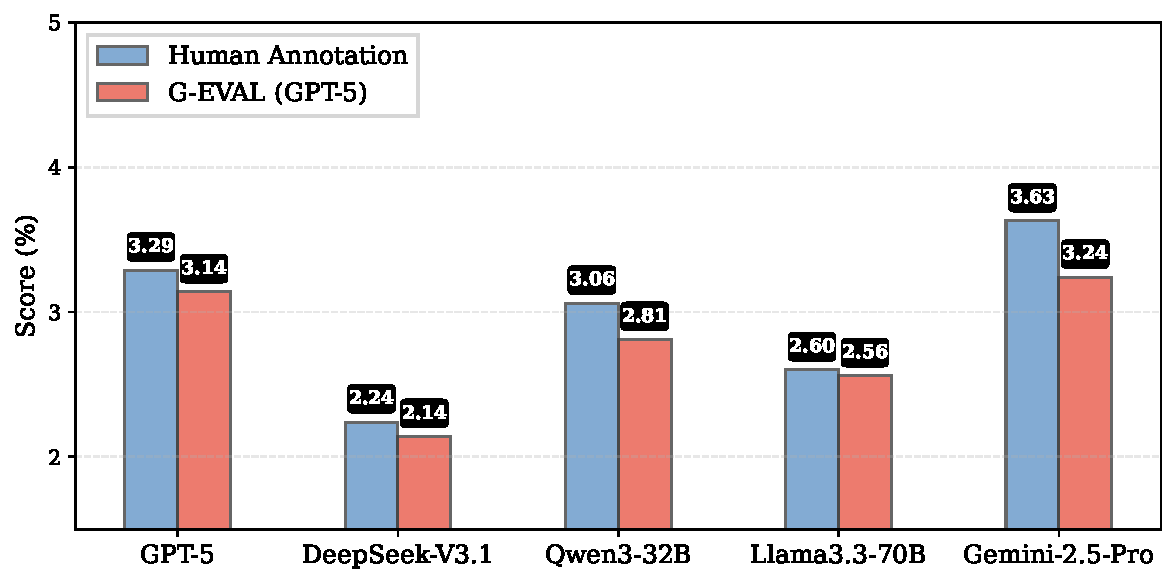
\includegraphics[width=1.0\linewidth]{Fig/score_across_model.pdf}
    % \vspace{-2.0em}
    \caption{ Comparison of average scores of causal explanation assigned by human annotators and the G-EVAL (GPT-5) judge across five models.
    }
    \label{appendix_score_across_model}
\end{figure}

\begin{figure}[!ht]
  \centering
    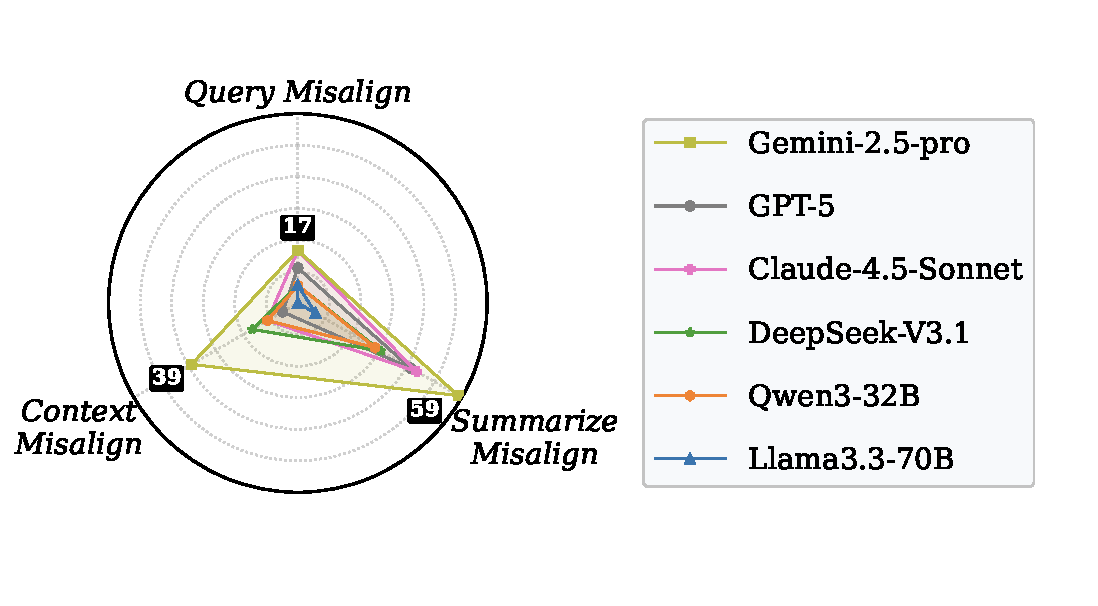
\includegraphics[width=1.0\linewidth]{Fig/agent_subcategory_retrieval_radar.pdf}
    % \vspace{-2.0em}
    \caption{ Step localization accuracy of six LLM judges across three retrieval hallucination subcategories.
    }
    \label{appendix_subcategory_retrieval}
\end{figure}

\begin{figure}[!ht]
  \centering
    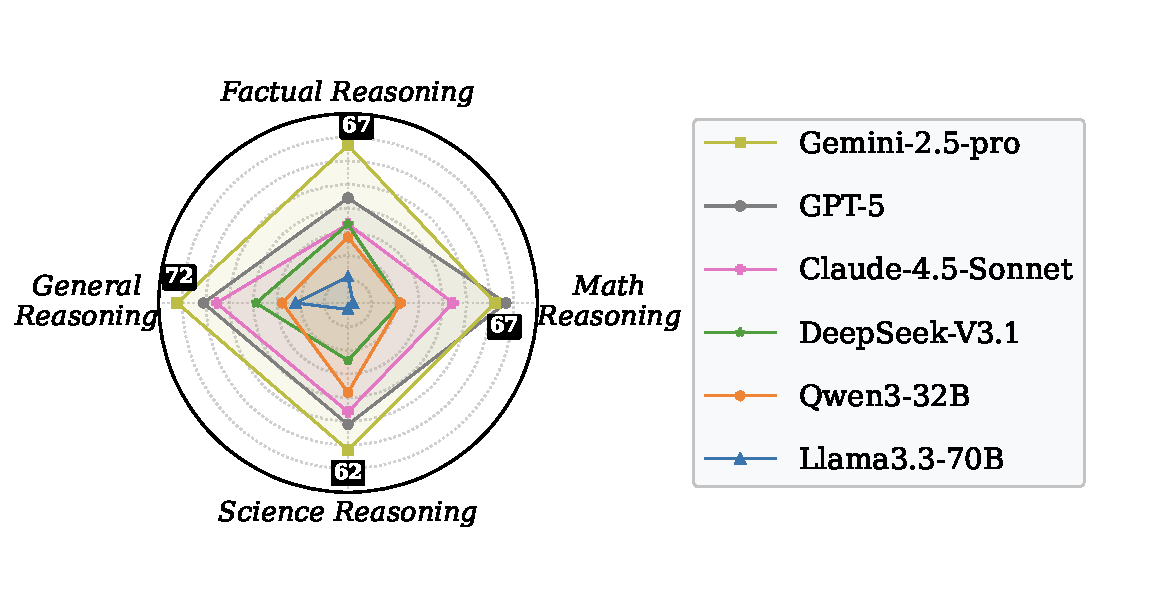
\includegraphics[width=1.0\linewidth]{Fig/agent_subcategory_reasoning_radar.pdf}
    % \vspace{-2.0em}
    \caption{ Step localization accuracy of six LLM judges across four reasoning hallucination subcategories.
    }
    \label{appendix_subcategory_reason}
\end{figure}

\begin{figure}[!ht]
  \centering
    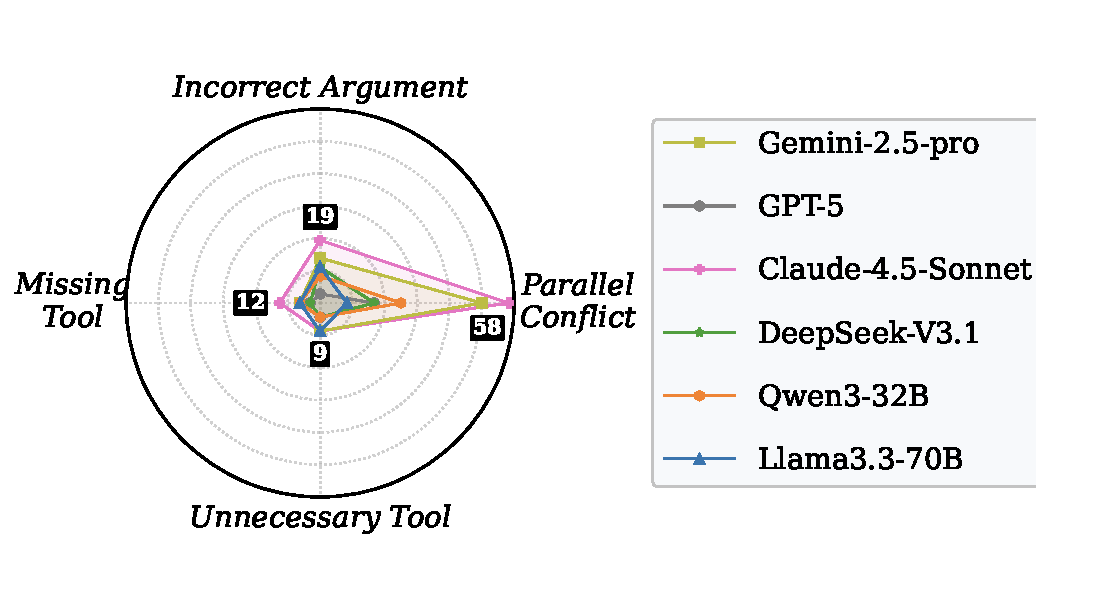
\includegraphics[width=1.0\linewidth]{Fig/agent_subcategory_tool_radar.pdf}
    % \vspace{-2.0em}
    \caption{ Step localization accuracy of six LLM judges across four tool-use hallucination subcategories.
    }
    \label{appendix_subcategory_tool}
\end{figure}

\subsection{More Analysis on Subcategories}
\label{appendix_subcategory_analysis}
We provide subcategory-level analysis for retrieval, reasoning, and tool-use hallucinations, described as follows:
\begin{itemize}[noitemsep,left=2pt, itemsep=0pt, topsep=0pt]
\item \textit{Analysis on Retrieval Hallucination}. 
We report step localization accuracy for each retrieval hallucination subcategory in Figure~\ref{appendix_subcategory_retrieval}. The results show that Gemini-2.5-Pro achieves the strongest attribution performance across the three retrieval-hallucination subcategories. 
Notably, Gemini-2.5-Pro shows a clear advantage in summarize misalign subcategory, indicating a superior ability to localize errors introduced during evidence aggregation and compression.
In contrast, the query misalign subcategory remains the most challenging for all models, suggesting that hallucinations seeded by an incorrect retrieval intent are harder to diagnose and more likely to be confounded with later steps.

\item \textit{Analysis on Reasoning Hallucination}. We report step localization accuracy for each reasoning hallucination subcategory in Figure~\ref{appendix_subcategory_reason}. Gemini-2.5-Pro consistently attains the highest accuracy across multiple hallucination reasoning subcategories. In contrast, open-source models perform substantially worse across all subcategories, indicating limited sensitivity to logical deviations. Overall, the results suggest that accurate reasoning-hallucination attribution requires fine-grained verification of intermediate claims and their dependencies, which remains a key bottleneck for current open-source models.

\item \textit{Analysis on Tool-Use Hallucination}. We report step localization accuracy for each tool-use hallucination subcategory in Figure~\ref{appendix_subcategory_tool}. The results indicate that all models perform poorly on most subcategories, including incorrect argument, missing tool, and unnecessary tool. In contrast, Claude-4.5-Sonnet identifies parallel conflict hallucinations with notably higher accuracy, suggesting that inconsistencies from concurrent tool executions yield more explicit and verifiable contradictions.
\end{itemize}

\section{More Details on Prompt Templates}

\subsection{Templates for Question-solving Paths}
Figure~\ref{appendix_question_solving_prompt} illustrates the prompt template used to instruct LLMs to construct detailed question-solving paths based on the question, the ground-truth answer, and, when available, dataset-provided solution annotations.

\begin{figure*}[!ht]
  \centering
    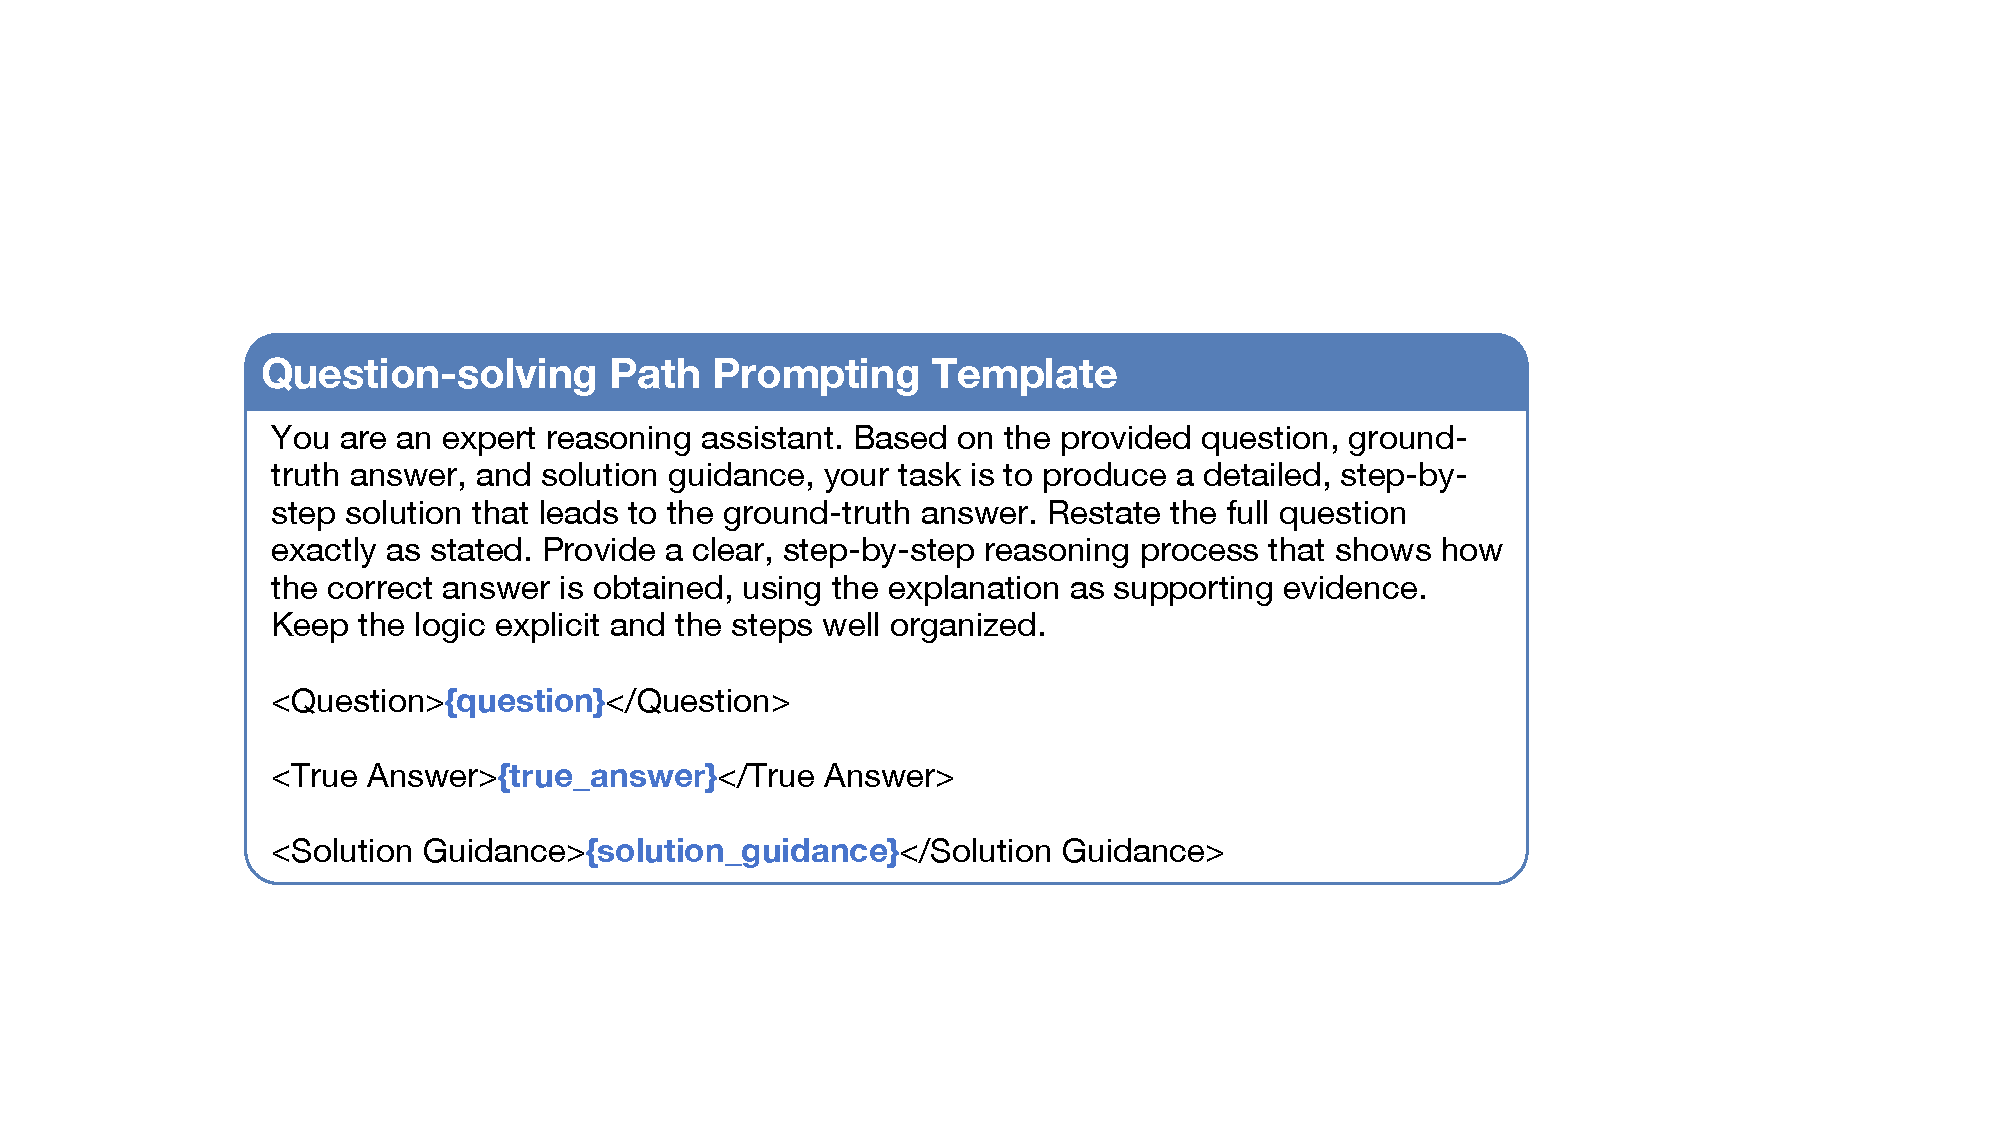
\includegraphics[width=0.95\linewidth]{Fig/qusetion_solution_prompt.pdf}
    % \vspace{-2.0em}
    \caption{ Prompt template for constructing question-solving paths. The ``question'', ``true\_answer'', and ``solution\_guidance'' placeholders are replaced with the corresponding query, the ground-truth answer and the dataset-provided solution annotations.
    }
    \label{appendix_question_solving_prompt}
\end{figure*}

\begin{figure*}[!ht]
  \centering
    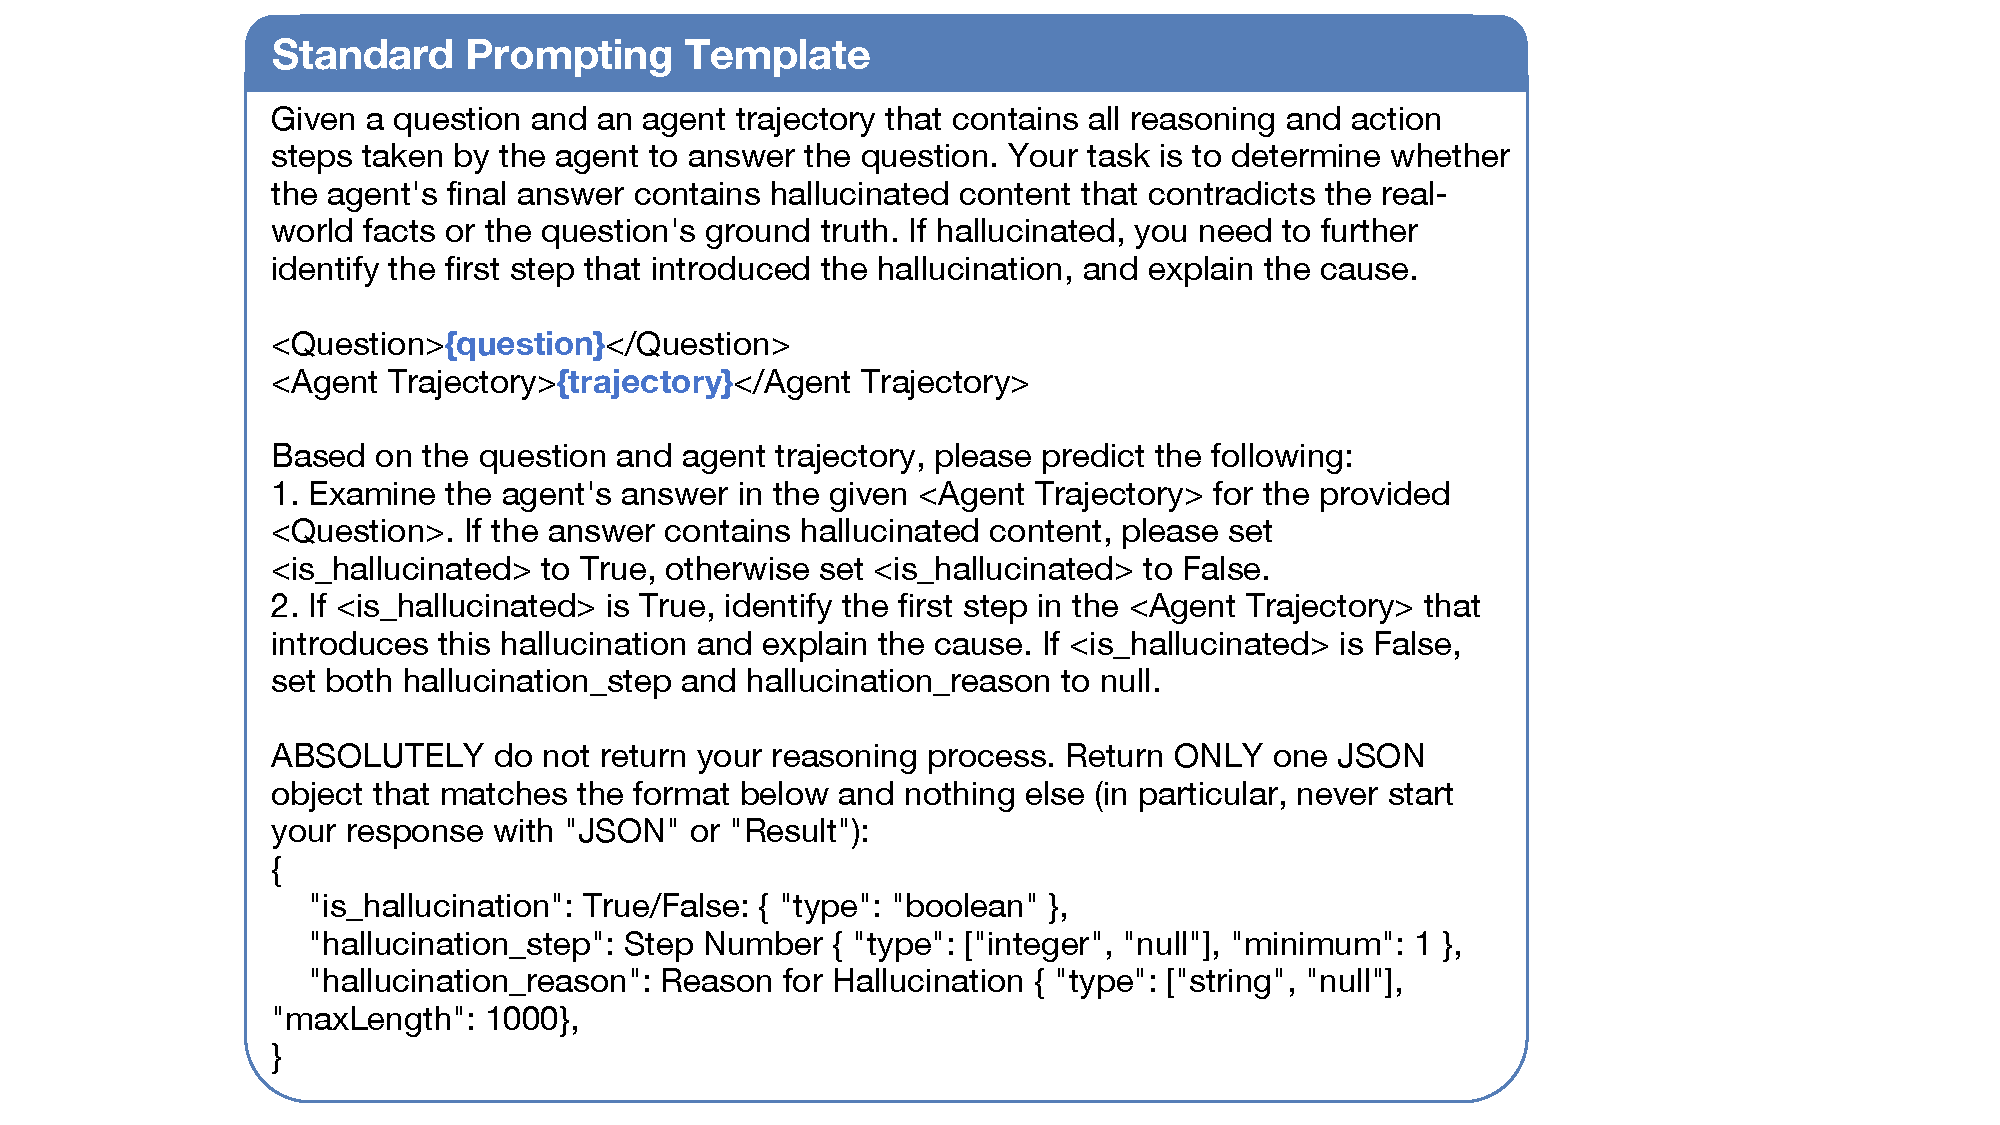
\includegraphics[width=0.95\linewidth]{Fig/standard_prompting_prompt.pdf}
    % \vspace{-2.0em}
    \caption{ Prompt template for automated hallucination judgment and attribution using standard prompting method. The ``question'' and ``trajectory'' placeholders are replaced with the corresponding query and agent trajectory to be evaluated.
    }
    \label{appendix_standard_prompting_prompt}
\end{figure*}

\begin{figure*}[!ht]
  \centering
    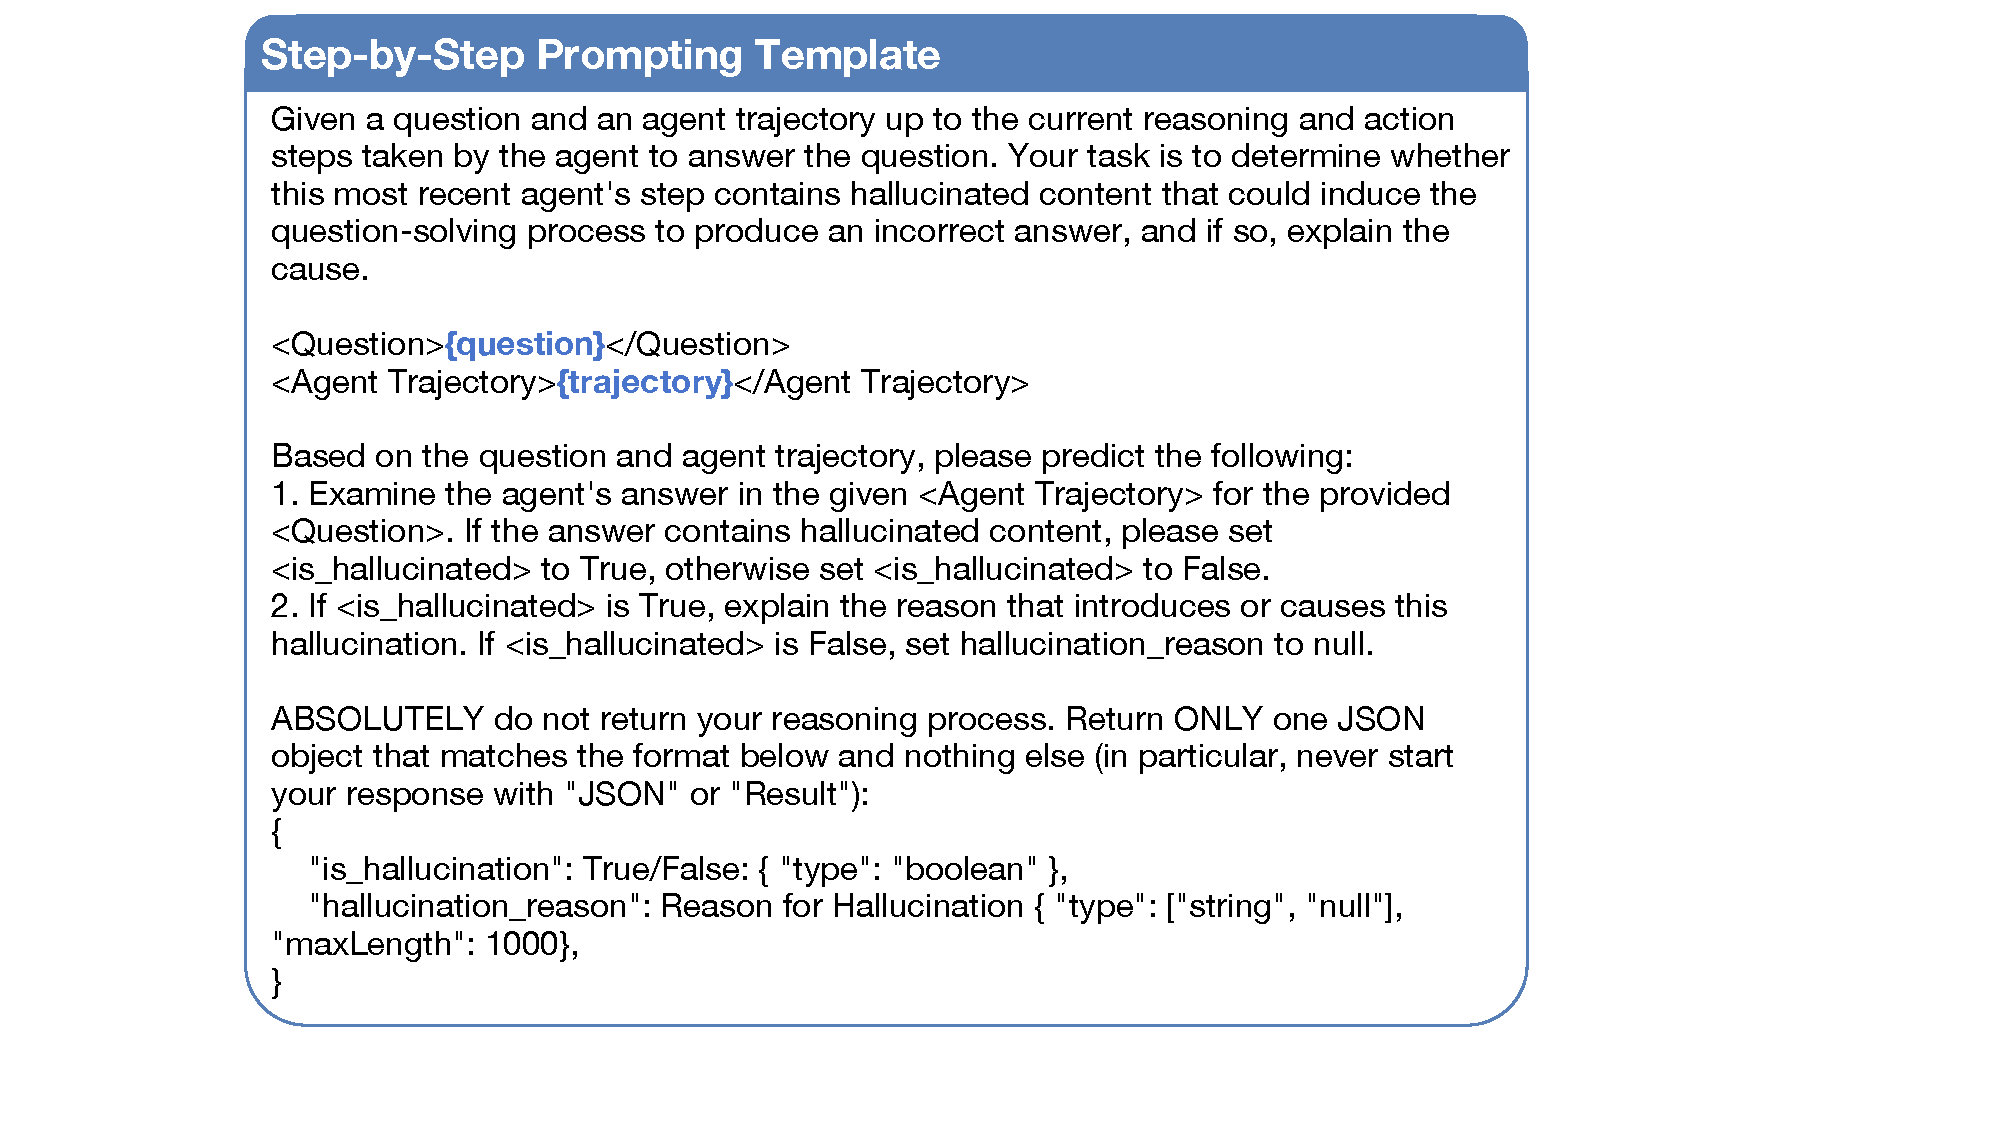
\includegraphics[width=1.0\linewidth]{Fig/step_by_step_prompt.pdf}
    % \vspace{-2.0em}
    \caption{ Prompt template for automated hallucination judgment and attribution using step-by-step prompting method. The ``question'' and ``trajectory'' placeholders are replaced with the corresponding query and agent trajectory to be evaluated.
    }
    \label{appendix_step_by_step_prompt}
\end{figure*}

\subsection{Templates for Standard Prompting}
Figure~\ref{appendix_standard_prompting_prompt} shows the prompt template for standard prompting, where the LLM is provided with the query and the full trajectory and instructed to perform hallucination judgment and attribution.

\subsection{Templates for Step-by-Step Prompting}
Figure~\ref{appendix_step_by_step_prompt} illustrates the prompt template for step-by-step prompting, where the model processes the query and trajectory incrementally, determines whether a hallucination occurs at each step, and stops once a hallucination is detected.

\subsection{Templates for G-EVAL Evaluation}
\label{appendix_prompt_geval}
Figure~\ref{appendix_geval_prompt} illustrates the prompt template for G-EVAL evaluation. We evaluate each model’s causal explanation, with reference to the trajectory and the human-annotated explanation. For each instance, G-EVAL assigns a five-point ordinal score under a fixed rubric that prioritizes explanation accuracy.


\section{Case Study}
In this section, we provide qualitative case analysis of agent hallucination attribution in Figures~\ref{appendix_case_planning},~\ref{appendix_case_retrieval},~\ref{appendix_case_reasoning},~\ref{appendix_case_human},~\ref{appendix_case_tool}. This analysis is essential for assessing both hallucination identification and the ability to explain where and why hallucinations arise in agentic workflows. To this end, we examine representative hallucination cases from five models, each illustrating a dominant hallucination pattern from one category: planning, retrieval, reasoning, human interaction, or tool use. For each case, we contrast the each model’s predicted hallucination judgment, responsible step, and causal explanation with human annotations, and analyze where causal tracing breaks down.

\begin{figure*}[!ht]
  \centering
    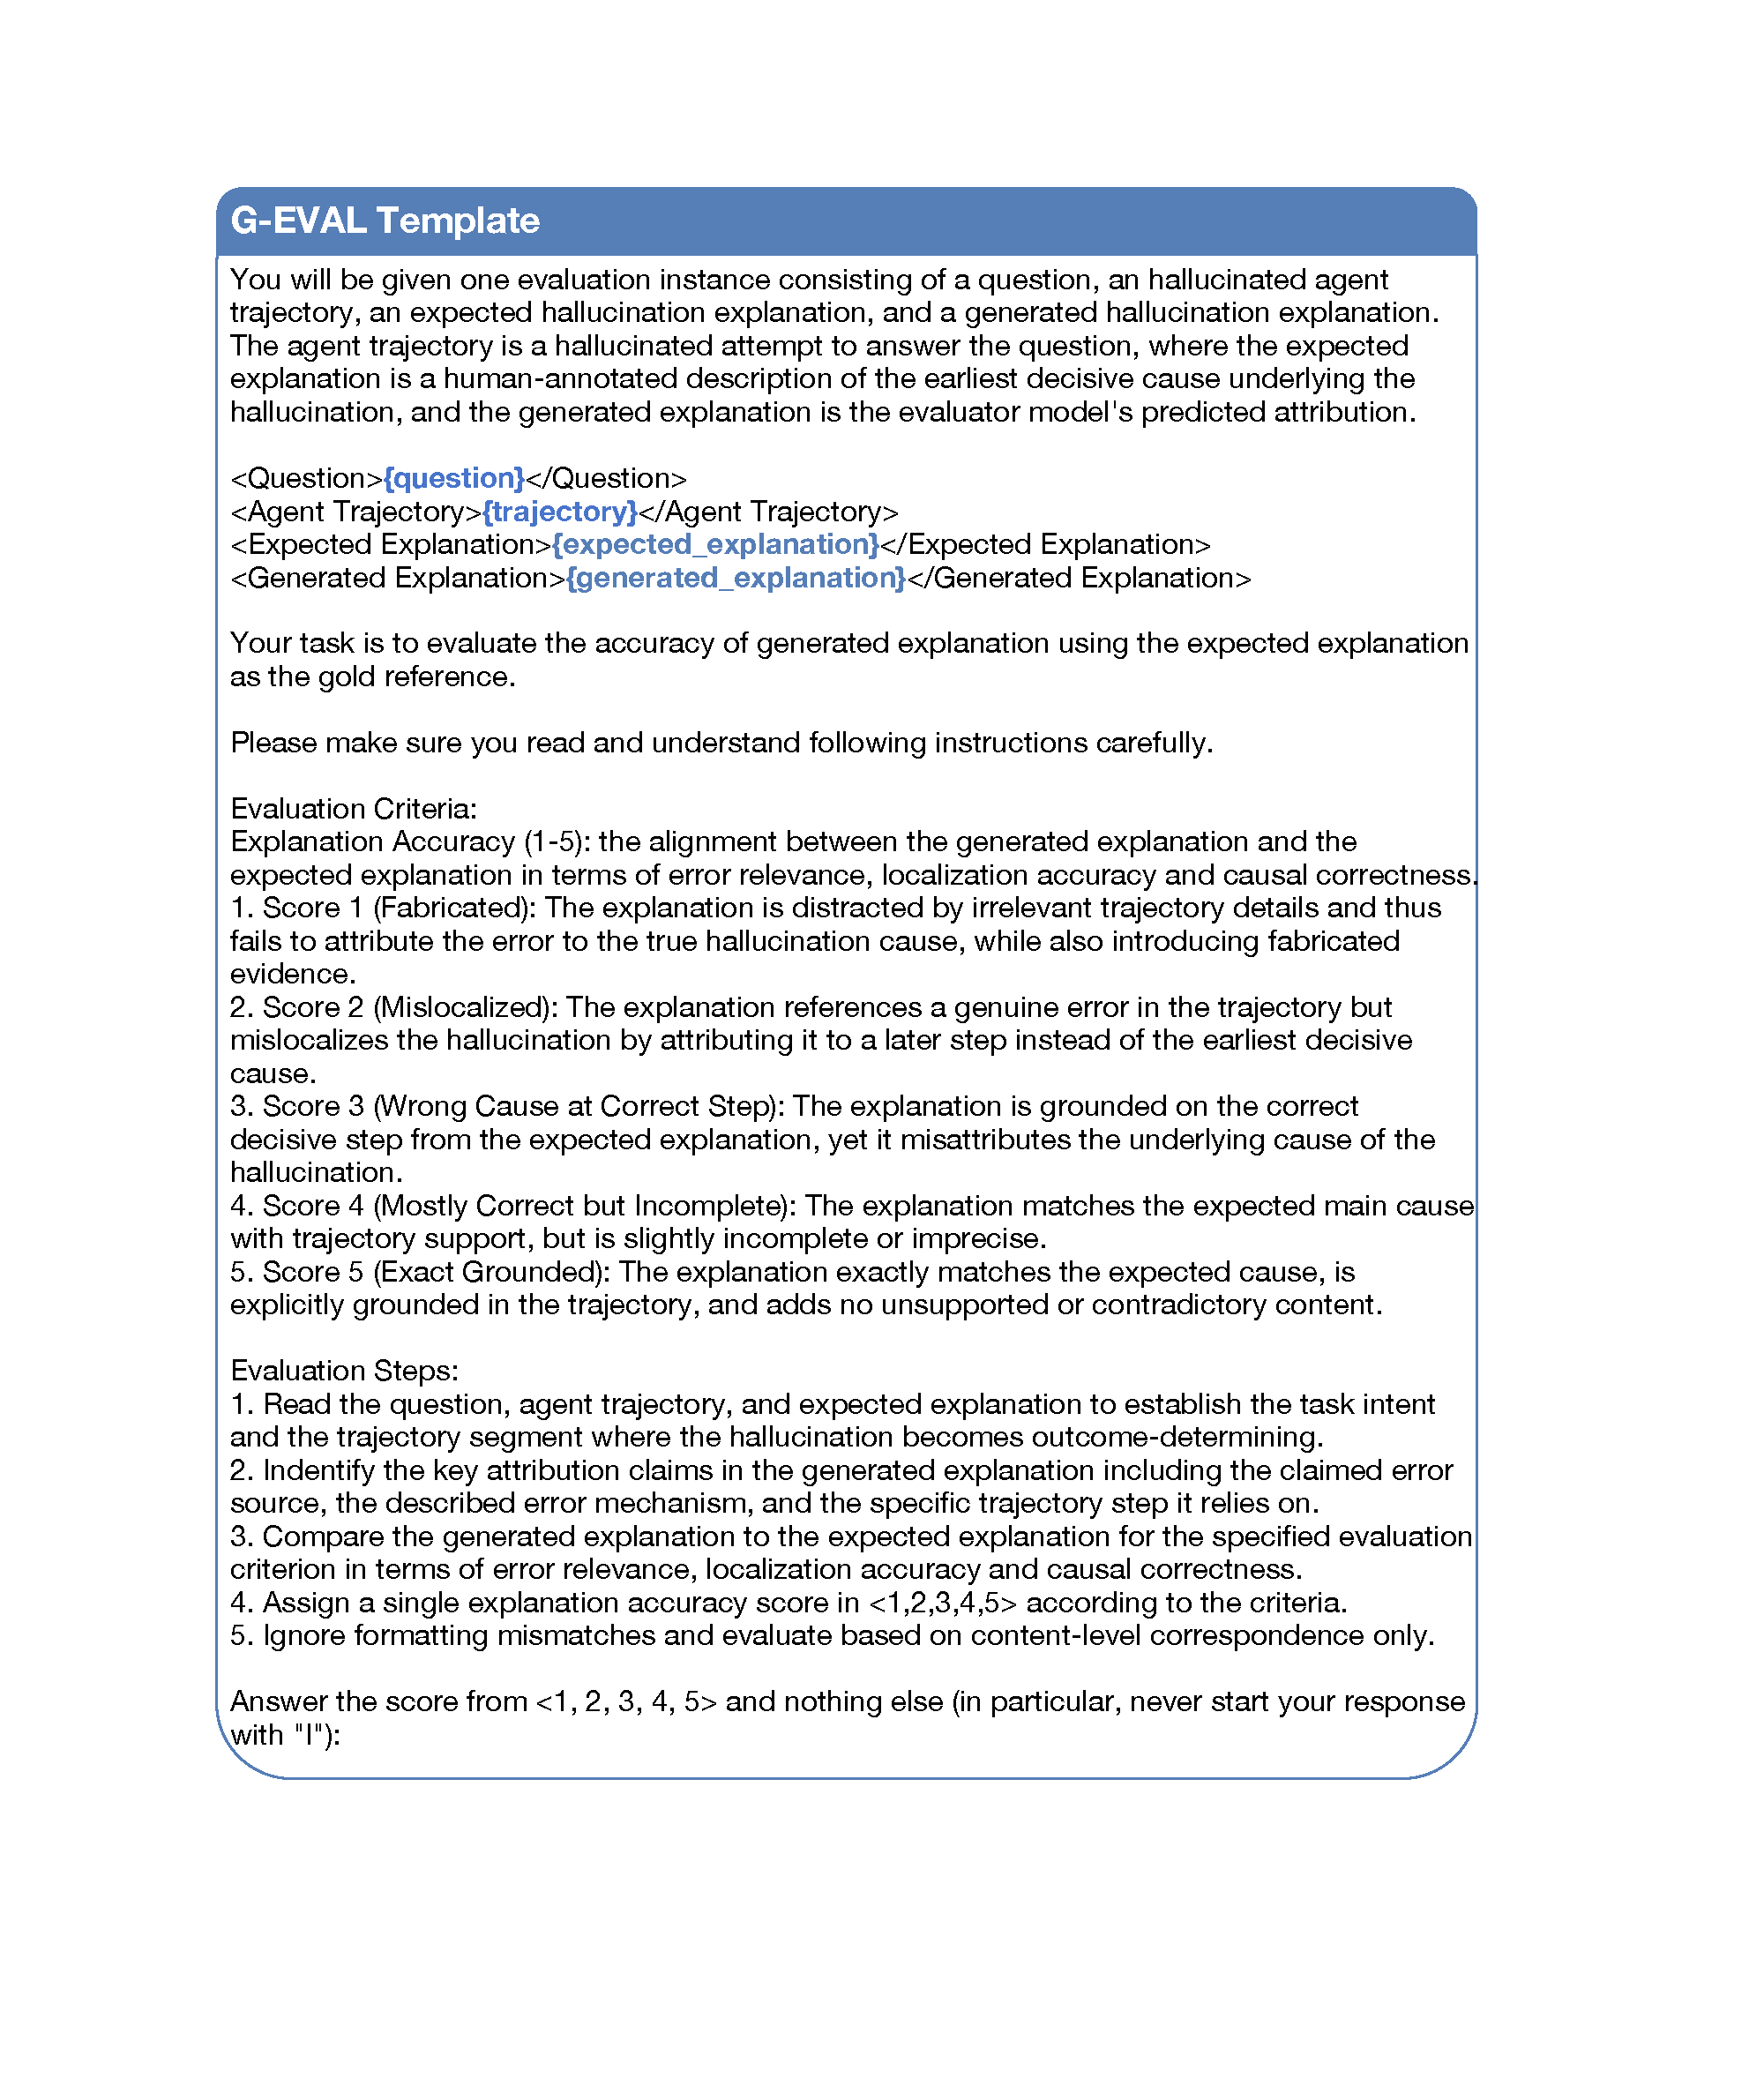
\includegraphics[width=1.0\linewidth]{Fig/geval_prompt.pdf}
    % \vspace{-2.0em}
    \caption{ Prompt template for explanation evaluation using G-EVAL method. The ``question'', ``trajectory'', ``expected\_explanation'' and ``generated\_explanation'' placeholders are replaced with the corresponding query, agent trajectory to be evaluated, the human-annotated expected explanation, and the explanation produced by the LLMs.
    }
    \label{appendix_geval_prompt}
\end{figure*}

\begin{figure*}[!ht]
  \centering
    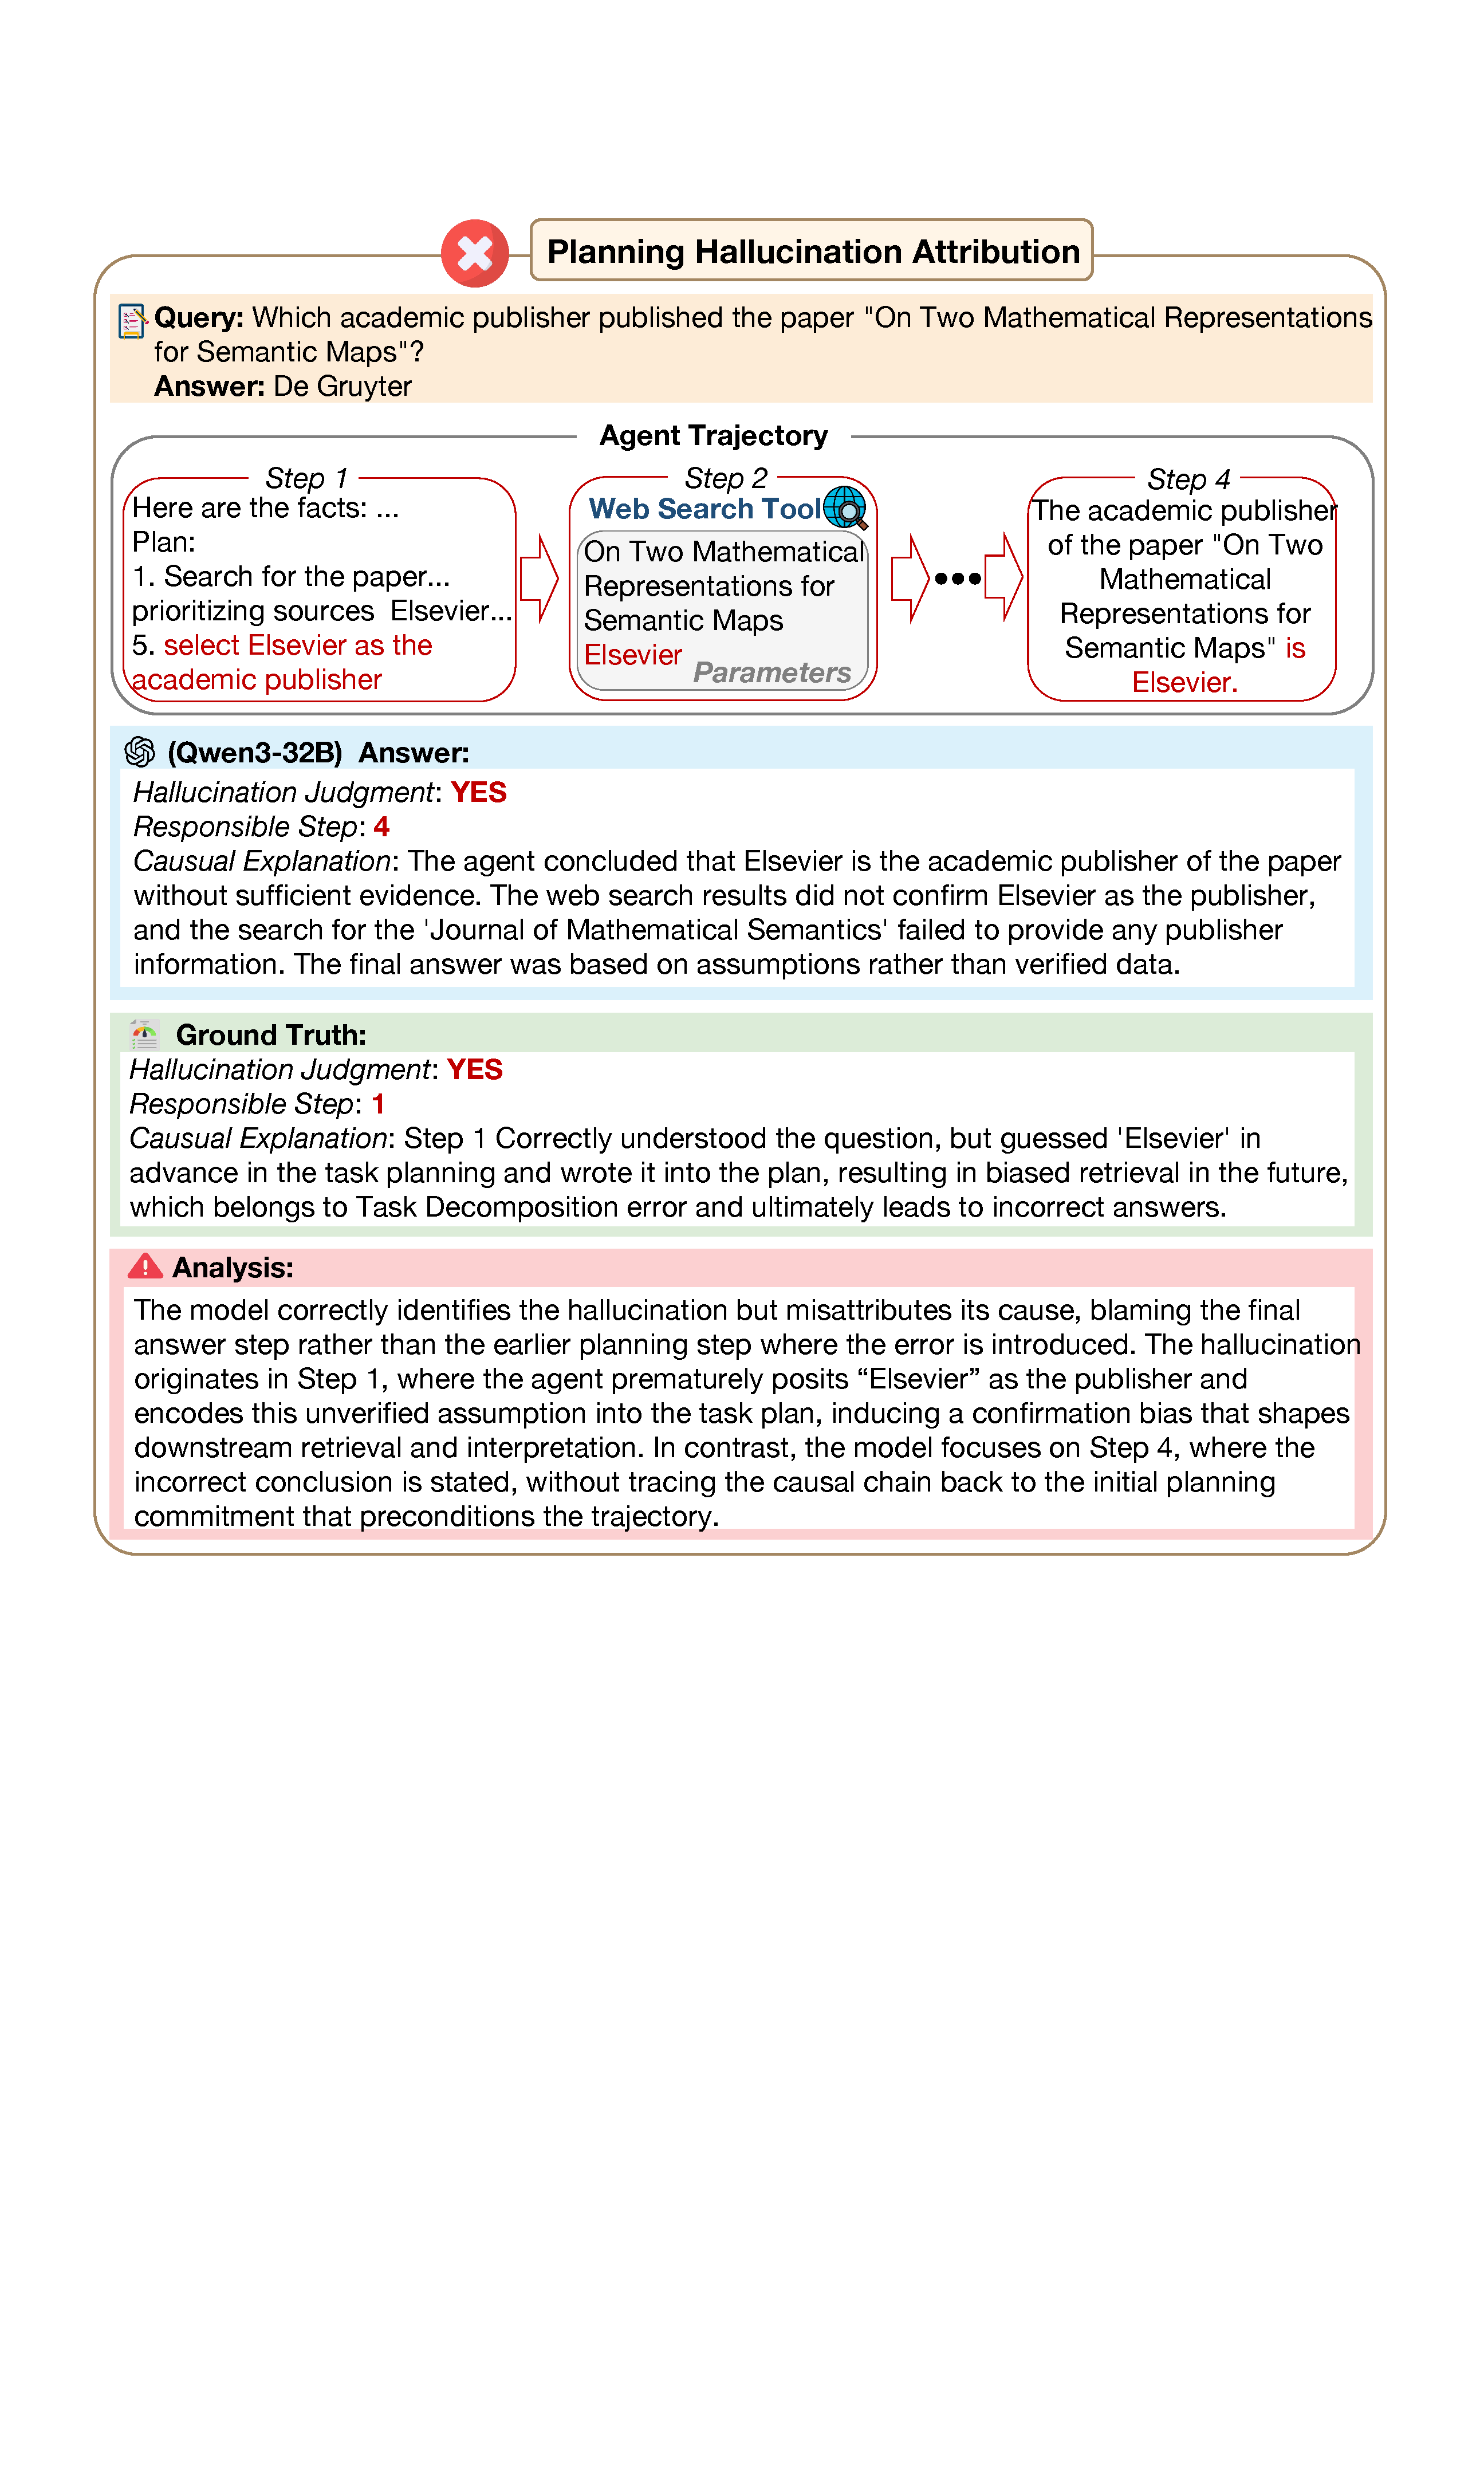
\includegraphics[width=1.0\linewidth]{Fig/case_analysis_planning.pdf}
    % \vspace{-2.0em}
    \caption{ Attribution example of planning hallucination category, with Qwen3-32B’s answers.
    }
    \label{appendix_case_planning}
\end{figure*}

\begin{figure*}[!ht]
  \centering
    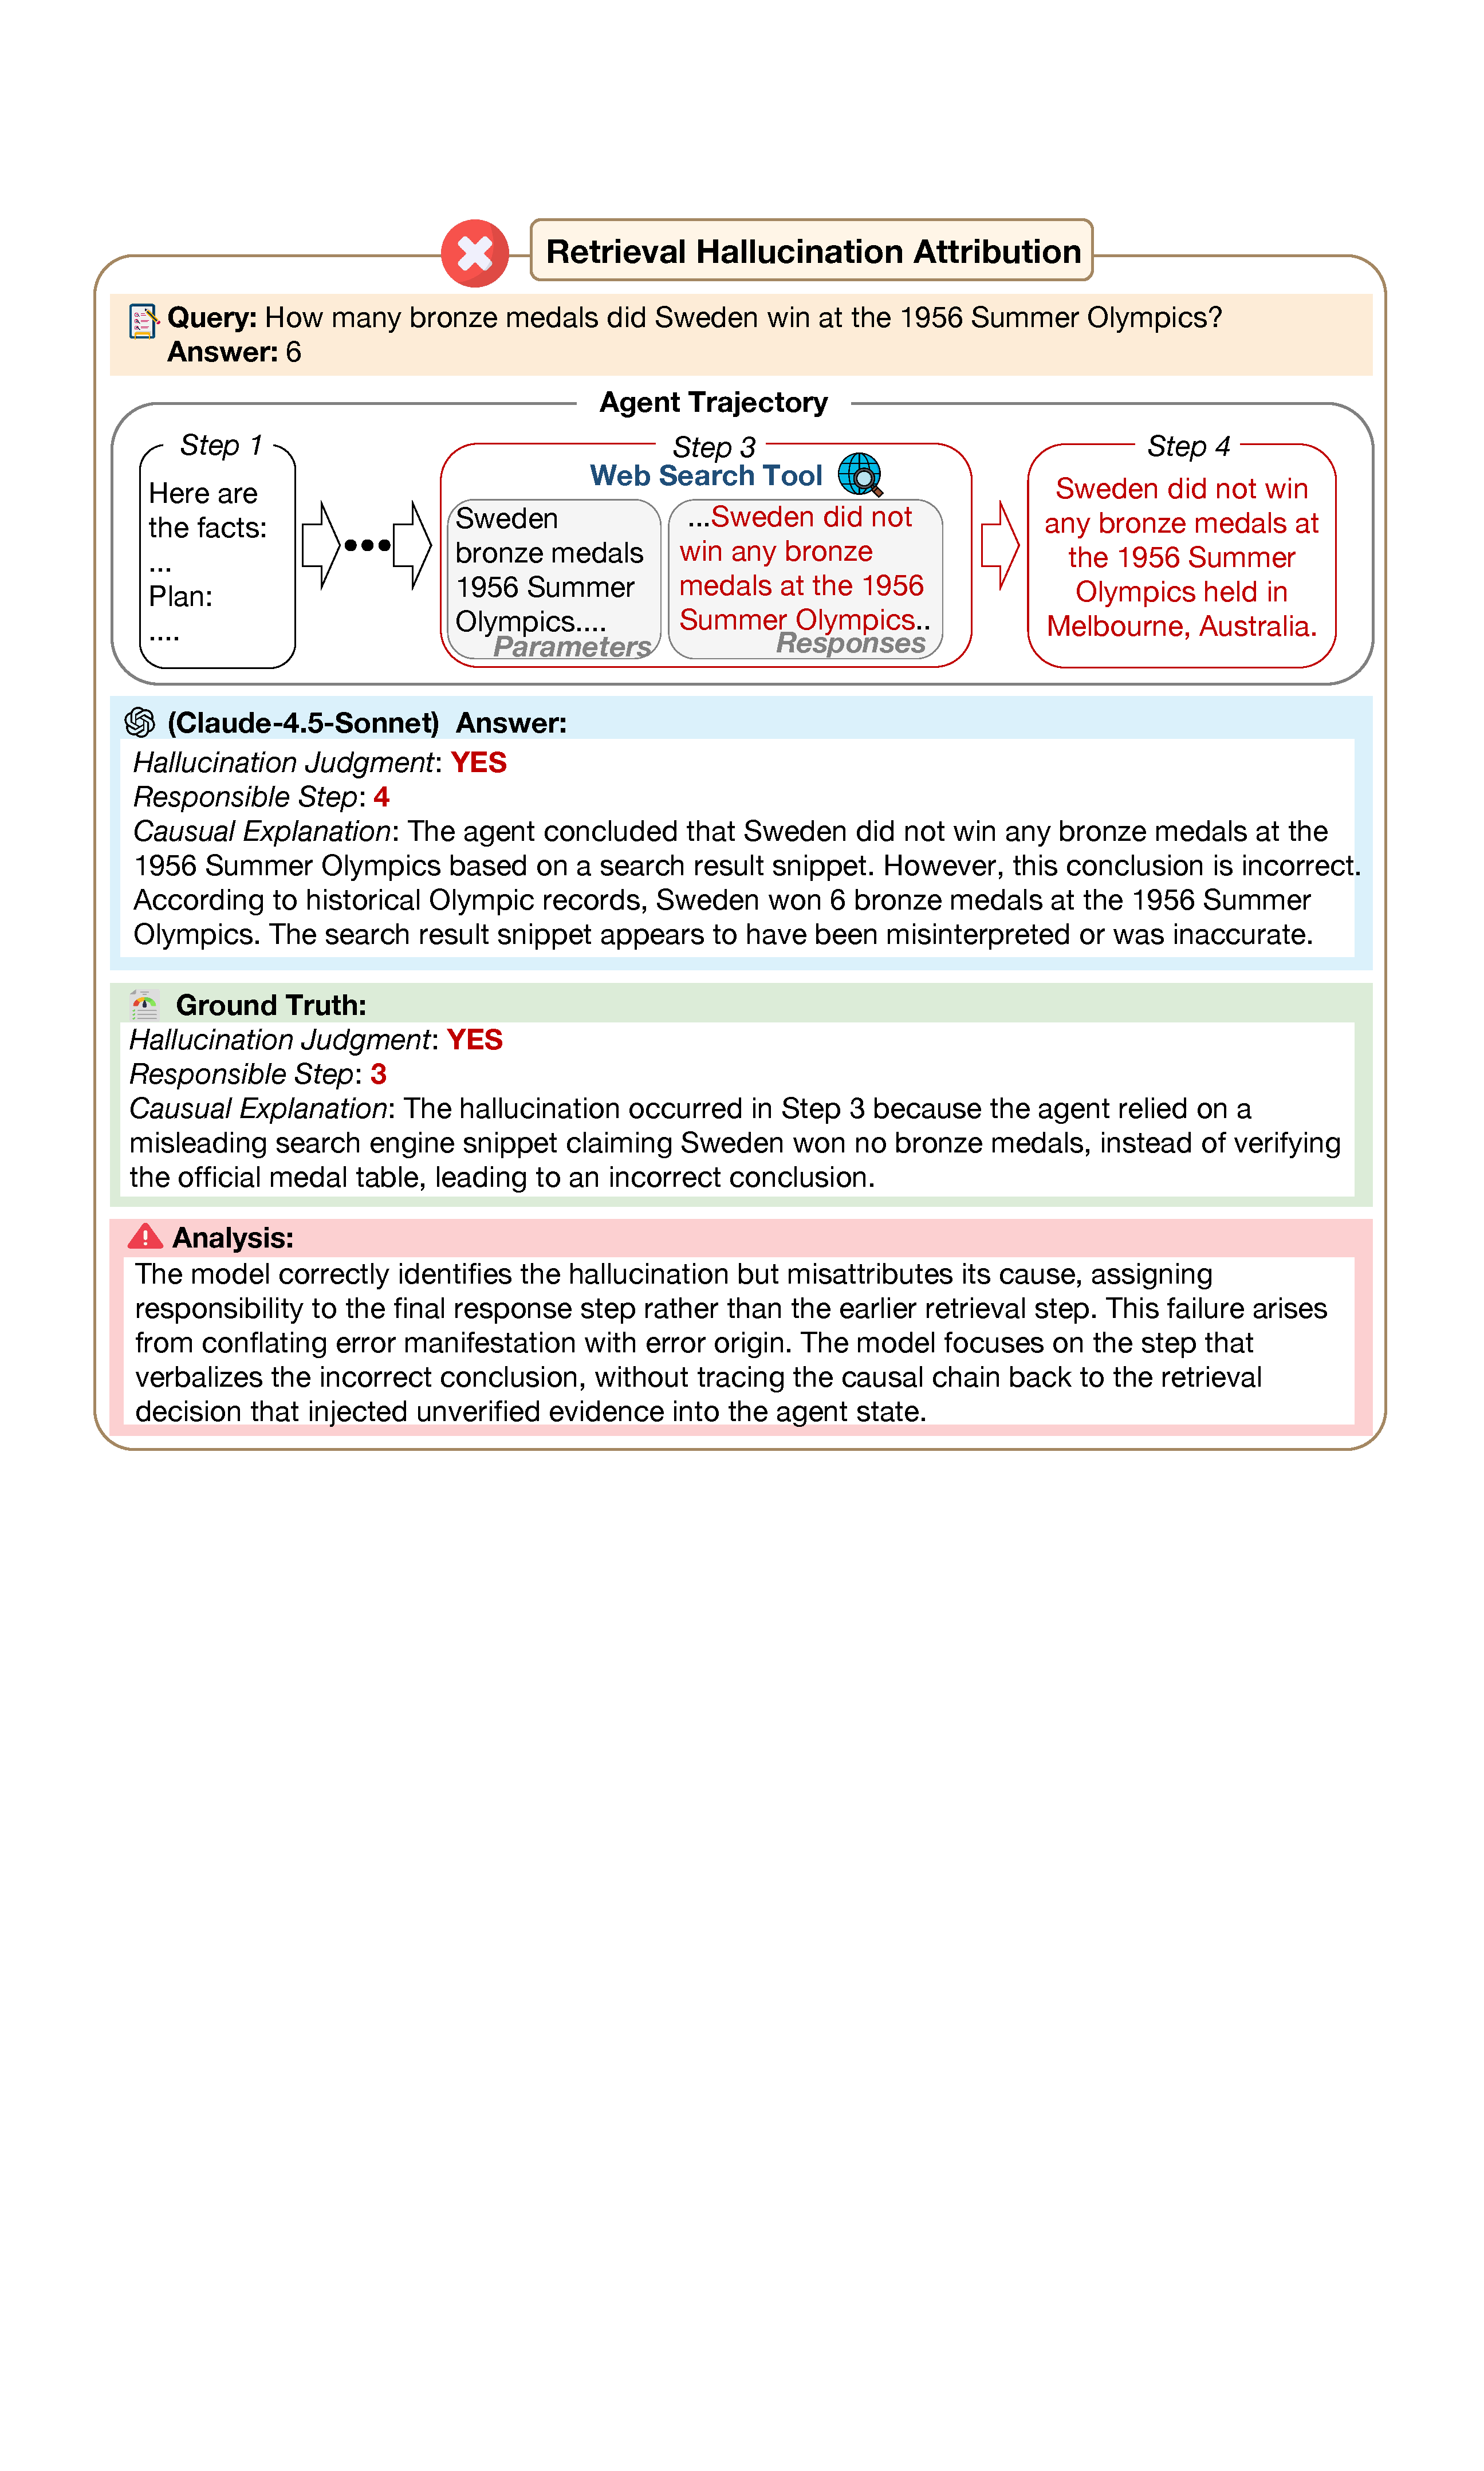
\includegraphics[width=1.0\linewidth]{Fig/case_analysis_retrieval.pdf}
    % \vspace{-2.0em}
    \caption{ Attribution example of retrieval hallucination category, with Claude-4.5-Sonnet’s answers. 
    }
    \label{appendix_case_retrieval}
\end{figure*}

\begin{figure*}[!ht]
  \centering
    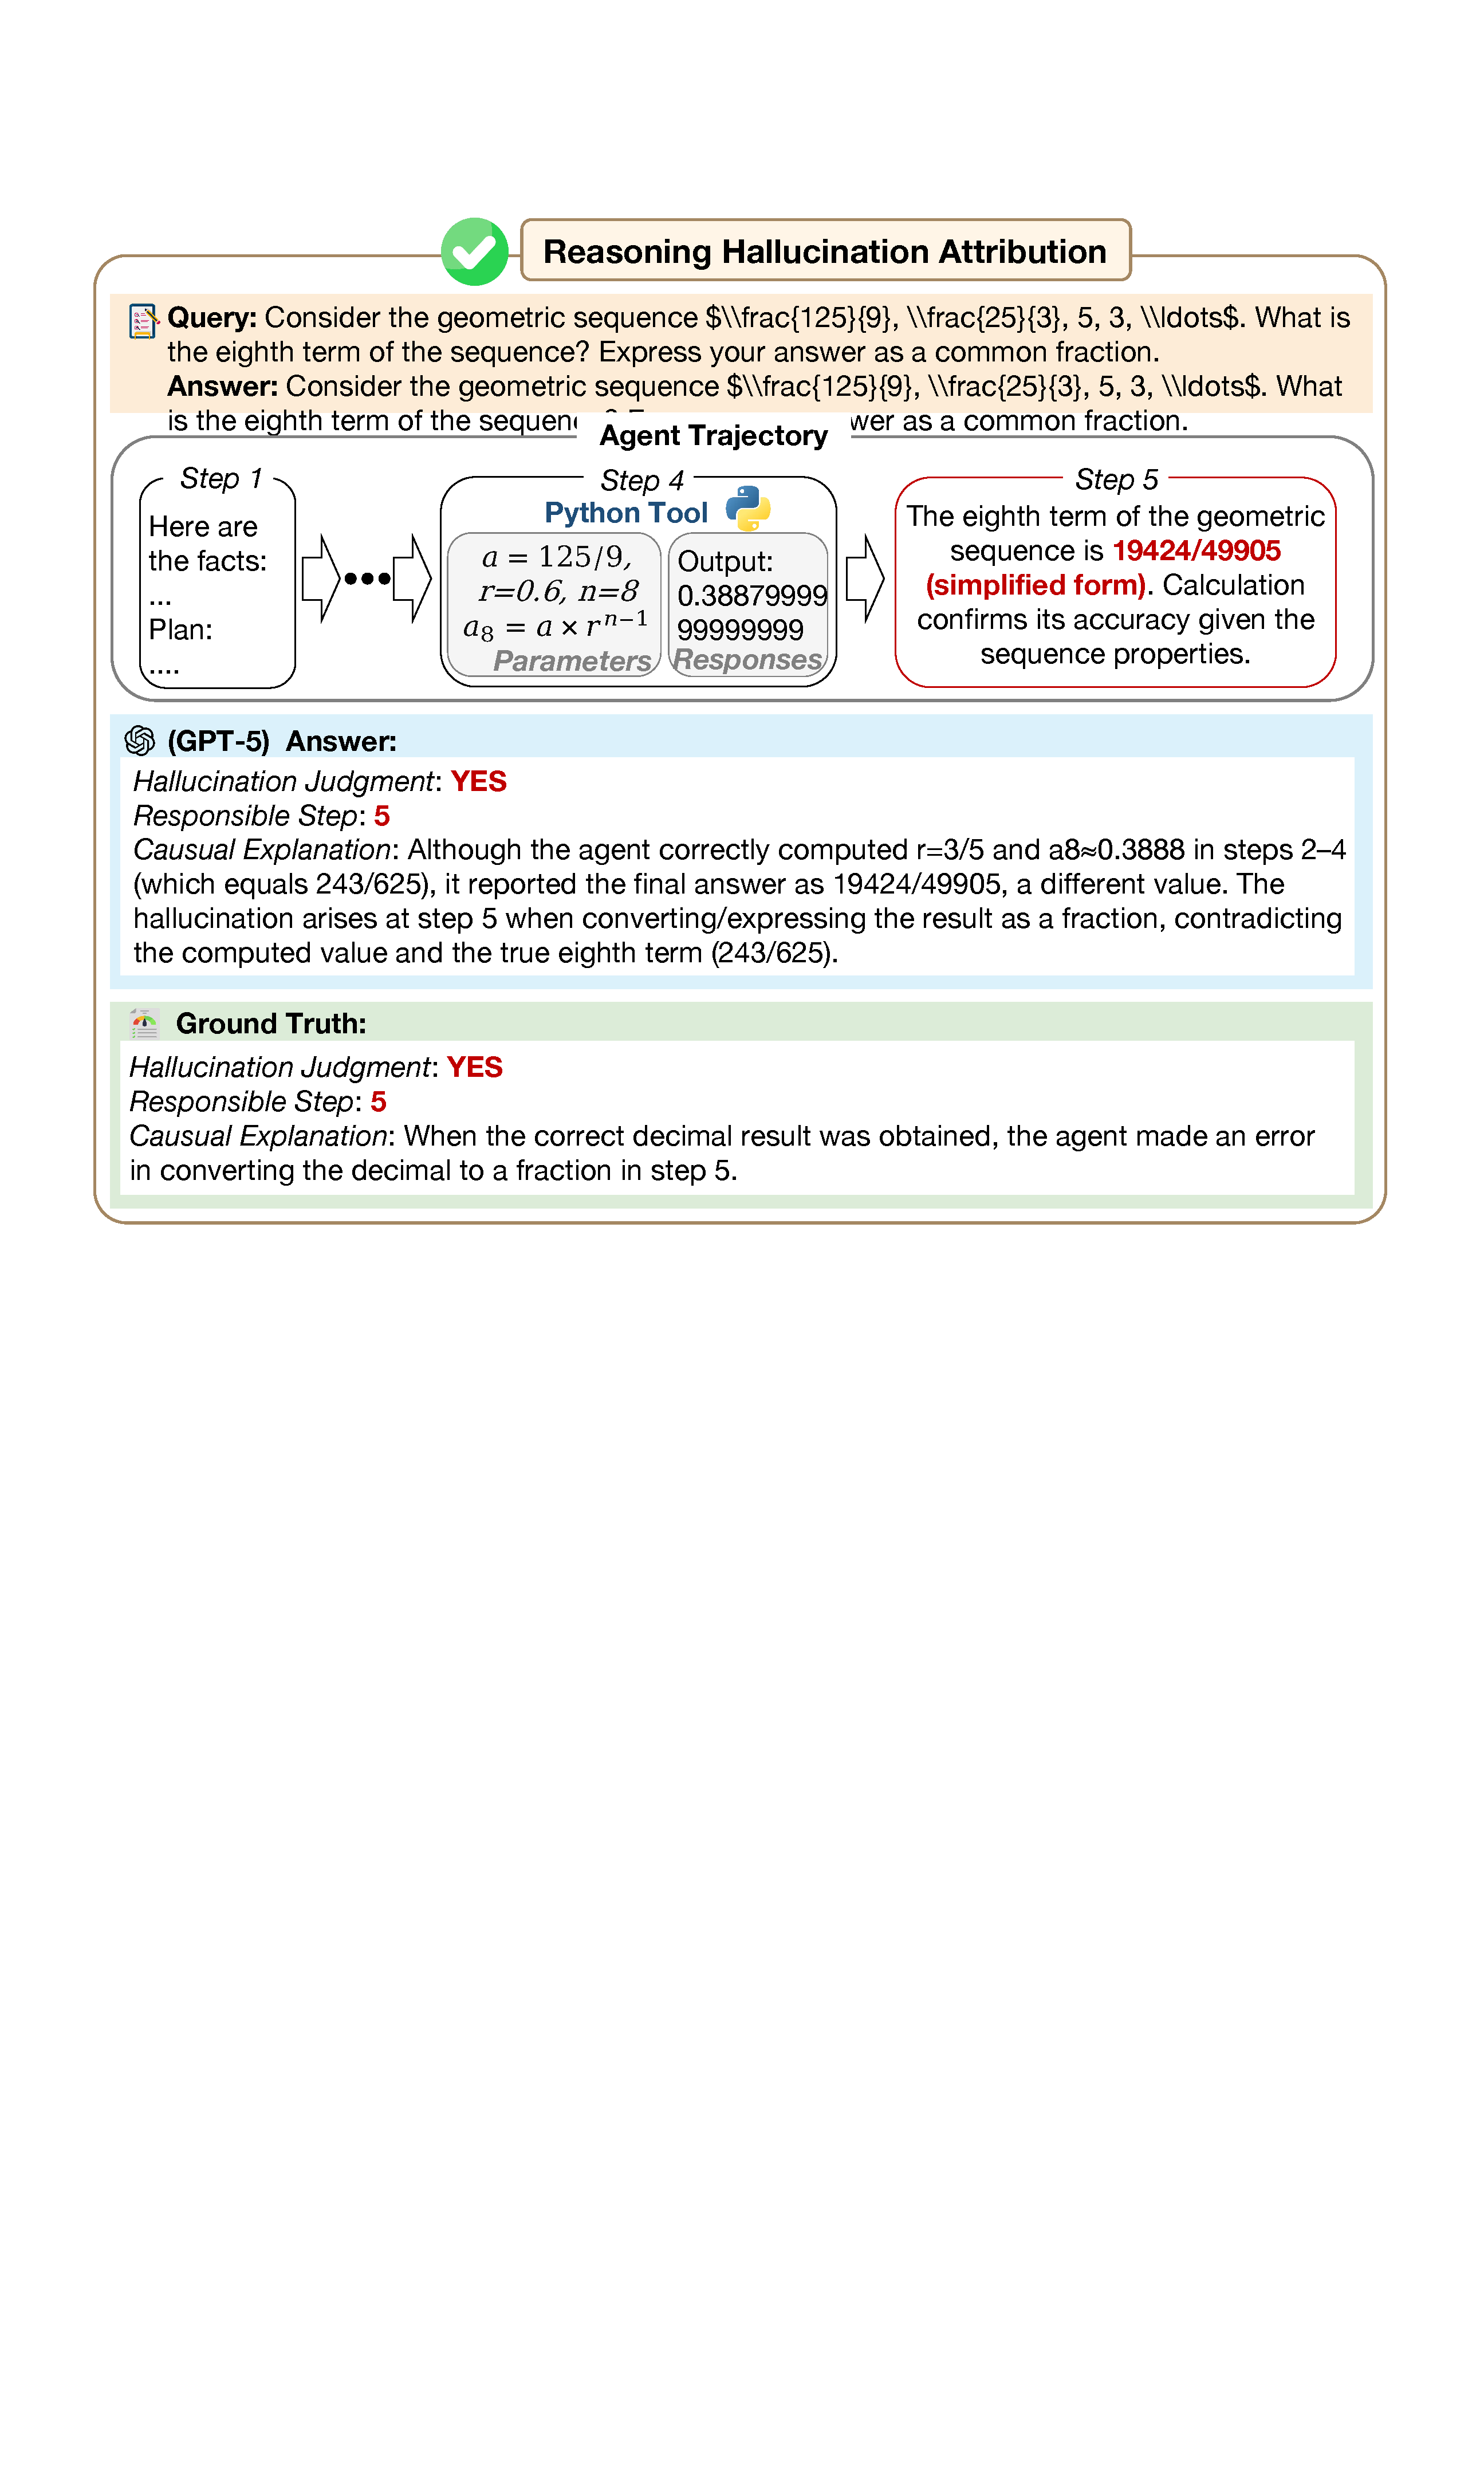
\includegraphics[width=1.0\linewidth]{Fig/case_analysis_reasoning.pdf}
    % \vspace{-2.0em}
    \caption{ Attribution example of reasoning hallucination category, with GPT-5’s answers.
    }
    \label{appendix_case_reasoning}
\end{figure*}

\begin{figure*}[!ht]
  \centering
    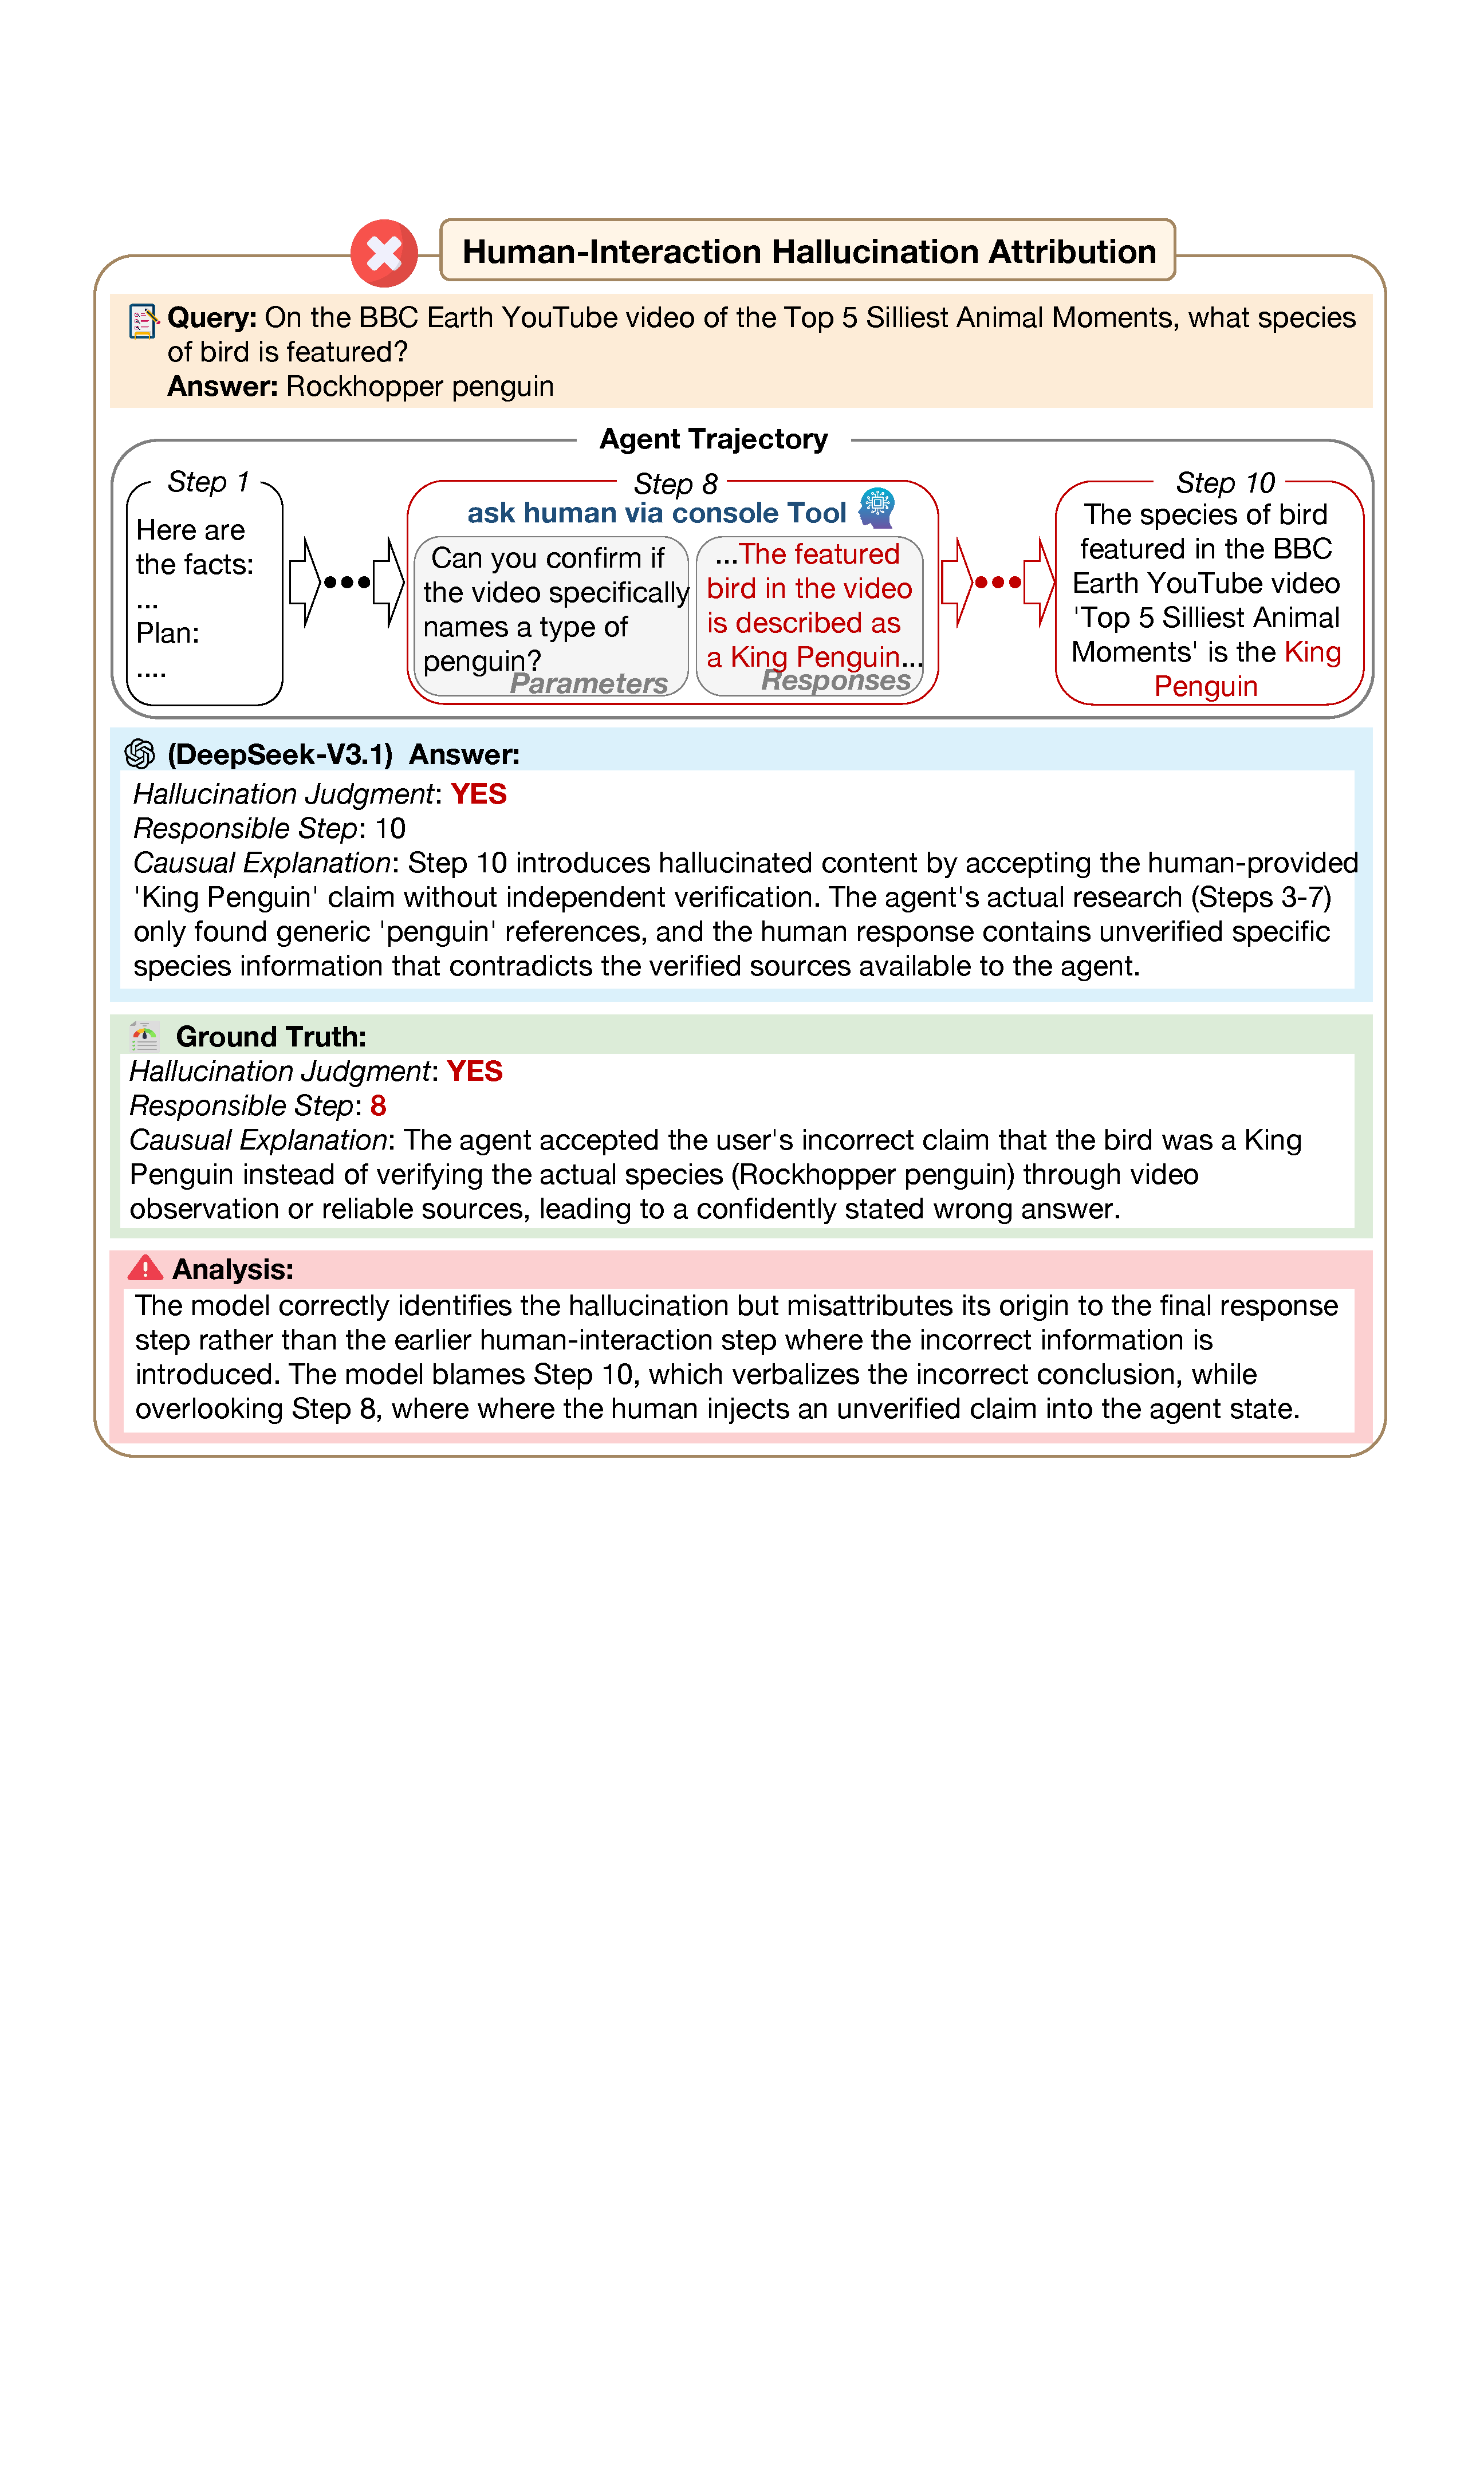
\includegraphics[width=1.0\linewidth]{Fig/case_analysis_human.pdf}
    % \vspace{-2.0em}
    \caption{ Attribution example of human-interaction hallucination category, with DeepSeek-V3.1’s answers.  
    }
    \label{appendix_case_human}
\end{figure*}


\begin{figure*}[!ht]
  \centering
    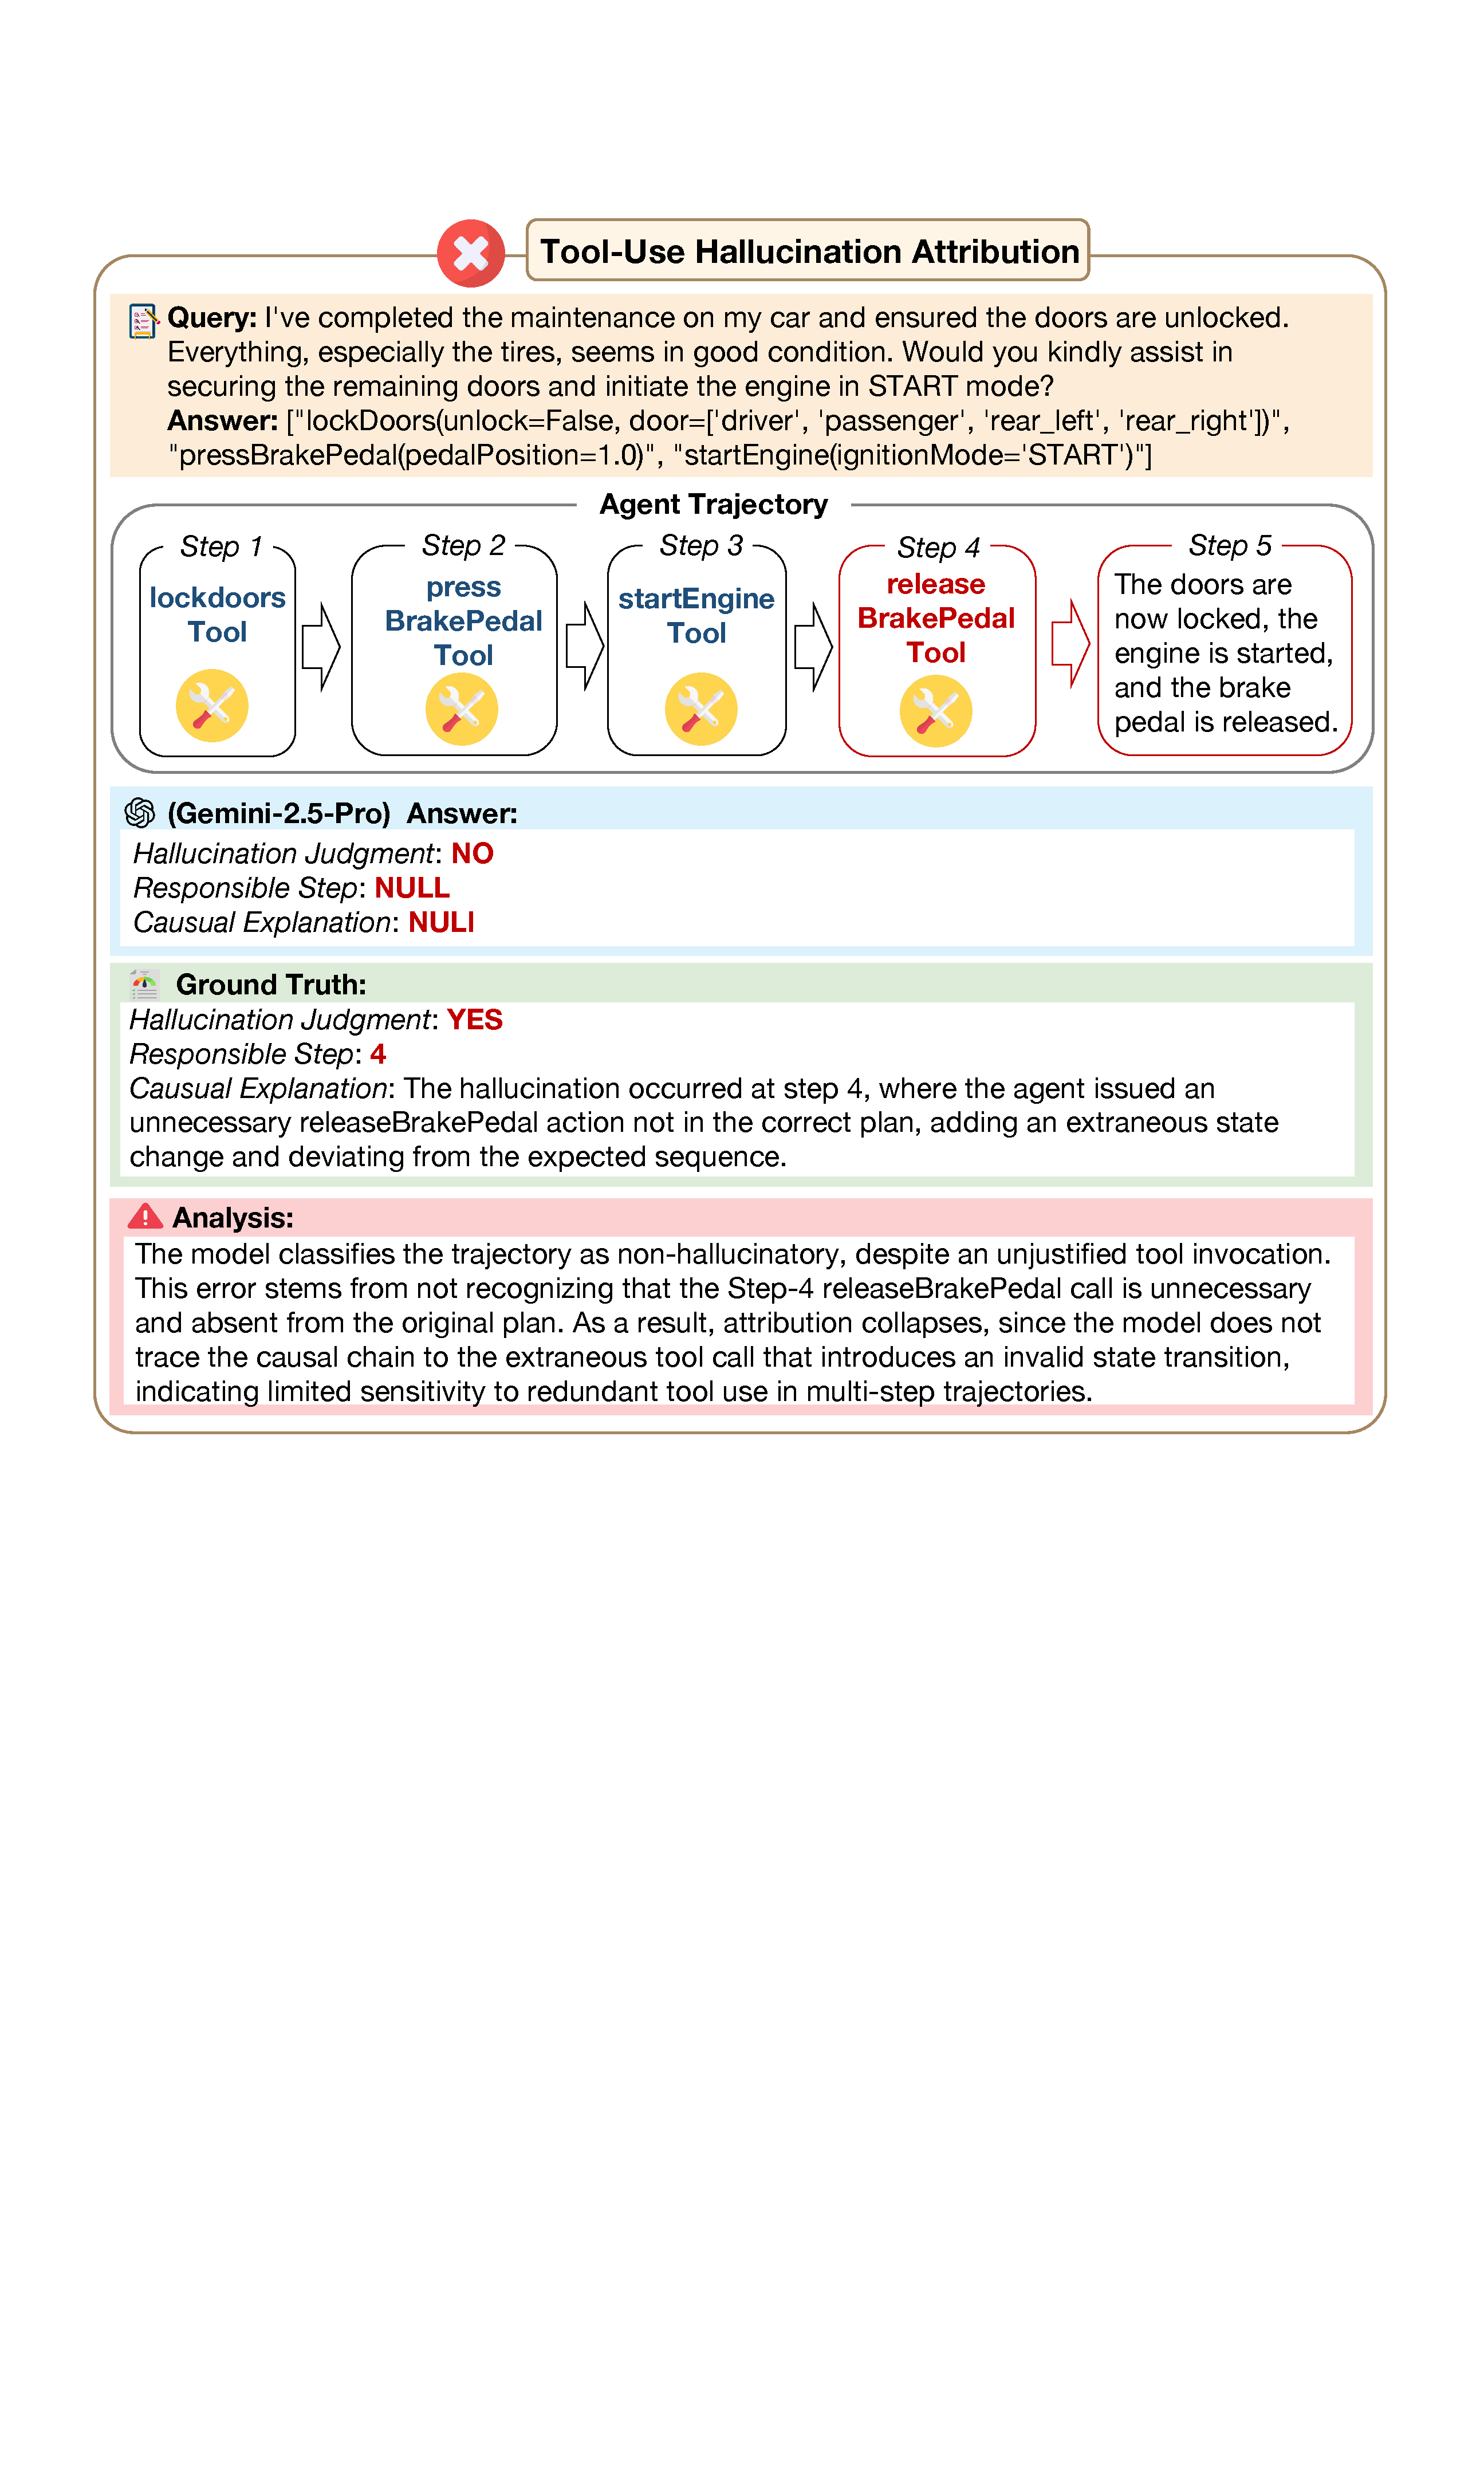
\includegraphics[width=1.0\linewidth]{Fig/case_analysis_tool.pdf}
    % \vspace{-2.0em}
    \caption{ Attribution example of tool-use hallucination category, with Gemini-2.5-Pro’s answers.  
    }
    \label{appendix_case_tool}
\end{figure*}

\section{Broader Impact}
AgentHallu aims to advance the reliability and transparency of LLM-based agents by enabling systematic hallucination diagnosis in multi-step workflows. By introducing a new task of automated hallucination attribution and providing a comprehensive benchmark with fine-grained annotations, AgentHallu enables researchers to better understand where and why hallucinations arise during agent execution. This capability is critical as LLM-based agents are increasingly deployed in high-stakes applications such as healthcare, finance, and decision support, where undetected error propagation can lead to severe downstream consequences.

We acknowledge the broader societal implications of releasing benchmarks for autonomous agents. AgentHallu is constructed exclusively from publicly available data and controlled agent executions, with all annotations carefully curated to avoid sensitive or harmful content. By emphasizing transparency, reproducibility, and ethical data practices, AgentHallu fosters responsible research and deployment of LLM-based agents, contributing to the long-term realization of reliable agentic systems.



